\documentclass{article}

% ── Packages ──────────────────────────────────────────────────────────────────
\usepackage[utf8]{inputenc}
\usepackage[T1]{fontenc}
\usepackage{microtype}          % better text rendering
\usepackage{amsmath,amssymb,amsfonts,amsthm}
\usepackage{mathtools}          % dcases, etc.
\usepackage{bm}                 % bold math
\usepackage{algorithm,algorithmic}
\usepackage{graphicx}
\usepackage{subcaption}
\usepackage{booktabs}
\usepackage{multirow}
\usepackage{xcolor}
\usepackage{hyperref}
\usepackage{cleveref}
\usepackage{natbib}
\usepackage{url}
% Page geometry: only active when compiling without neurips_2024.sty.
% neurips_2024.sty enforces its own margins; loading geometry after it is a no-op,
% but loading it before causes a conflict. We guard it here.
\IfFileExists{neurips_2024.sty}{}{%
  \IfFileExists{nips_2024.sty}{}{\usepackage[margin=1in]{geometry}}}

% NeurIPS style — use the version you have; fall back to plain article if absent
\IfFileExists{neurips_2024.sty}{\usepackage{neurips_2024}}{%
  \IfFileExists{nips_2024.sty}{\usepackage{nips_2024}}{}}

% ── Macros ────────────────────────────────────────────────────────────────────
\newcommand{\E}{E_{\bm\theta}}
\newcommand{\Etrue}{E^*}
\newcommand{\sE}{\mathcal{E}}
\newcommand{\R}{\mathbb{R}}
\newcommand{\xx}{\mathbf{x}}
\newcommand{\uu}{\mathbf{u}}
\newcommand{\ff}{\mathbf{f}}
\newcommand{\bphi}{\bm\phi}
\newcommand{\eps}{\varepsilon}
\newcommand{\norm}[1]{\left\|#1\right\|}
\newcommand{\abs}[1]{\left|#1\right|}
\DeclareMathOperator*{\argmin}{arg\,min}
\newtheorem{proposition}{Proposition}

% ── Title / Author ────────────────────────────────────────────────────────────
\title{%
  KAN-Parameterized Energy-Based Models\\
  Enable Controllable Test-Time Compute%
}

\author{%
  Hafez Khatib \\
  Department of Electrical and Computer Engineering \\
  American University of Beirut \\
  Beirut, Lebanon \\
  \texttt{hafezkhatib.2002@gmail.com}
}

\begin{document}
\maketitle

% ══════════════════════════════════════════════════════════════════════════════
\begin{abstract}
% ══════════════════════════════════════════════════════════════════════════════
The dominant deep-learning paradigm computes a fixed-cost function from input to output,
capping accuracy at model capacity rather than at available test-time budget. Energy-based
models (EBMs) supply an alternative --- iterative gradient descent on a learned scalar energy
--- but two obstacles remain: classical MLP-parameterised energies fail to support useful
iterative refinement at small parameter counts, and the \emph{peak-and-degrade} phenomenon
(additional inference compute eventually destroys the reconstruction) has been observed in
the literature but not quantified. We address both with \textbf{KAN-EBM}, an architecture
pairing a learned spatial filter bank with a Kolmogorov-Arnold Network as a
B-spline-parameterised energy.

Two empirical contributions follow. \textbf{(i)~The parameter--compute Pareto frontier.} On
CelebA-64 our $32$\,K-parameter KAN-EBM exceeds a fair-compute-matched MLP-EBM with $100\times$
more parameters by $+6.83$\,dB and a feed-forward DSM denoiser with $410\times$ more parameters
by $+4.55$\,dB at peak; on CIFAR-10 the same architecture occupies the low-parameter corner
of the parameter--compute Pareto frontier. \textbf{(ii)~An empirical scaling law for the
optimal inference depth.} We find $K^{*}(\sigma) \approx 86.7\,\sigma^{1.53}$
($R^{2}{=}0.98$ on CIFAR-10), beating four spectral predictors including a slow-mode timescale
derivation that fits with the \emph{wrong sign}. The law is invariant across a $19\times$
parameter range and three B-spline orders, generalises to CelebA-64 ($\alpha{=}1.36$),
but is \emph{not exhibited} by a fair-compute MLP-EBM ($R^{2}{=}0.42$): test-time-compute
scaling is a property of B-spline-parameterised energies, not a generic feature of EBM
gradient descent. The law collapses on Gaussian-blur deblurring, identifying i.i.d.-noise
corruption as its domain of validity. We provide a deployable early-stopping rule that
recovers $99.4\%$ of the oracle peak PSNR with no held-out validation. Theoretically:
Allen-Cahn gradient flow, score following under an EBM density, and predictive-coding error
minimisation are three constructions of a single update operator
$u\!\mapsto\!u-\eta\nabla E(u)$ for any smooth $E$, with a closed-form Gaussian special
case verified to floating-point precision.
\end{abstract}

% ══════════════════════════════════════════════════════════════════════════════
\section{Introduction}
% ══════════════════════════════════════════════════════════════════════════════

The dominant inference paradigm in deep learning is one-shot: a fixed-capacity model
maps input to output in a single forward pass, and accuracy improves only by increasing
model size. Recent work on language models shows that allocating additional
inference-time compute---through search, sampling, or iterative refinement---can match
or surpass gains from doubling parameter count \citep{snell2024llm}. A principled
\emph{architectural} mechanism for this trade-off has been absent in the vision domain.

\textbf{Energy-based models (EBMs)} offer exactly this mechanism: define a scalar
energy $E_\theta(\xx)$ over data space, train it so that $E$ is low near the data
manifold, and at inference run gradient descent $\xx_{t+1} = \xx_t - \eta\,\nabla_{\xx}
E_\theta(\xx_t)$ for $K$ steps. More steps $\Rightarrow$ better optimization of $E$
$\Rightarrow$ higher-quality reconstruction—naturally. However, scaling test-time compute
is bottlenecked by the parameter bloat of modern architectures. While EBMs offer a
natural framework for iterative inference, minimizing their parameter count traditionally
results in topological collapse of the energy basin. When a feedforward MLP is shrunk
to the microscopic parameter regime, its piecewise-linear activations (ReLU) create
jagged, non-navigable landscapes filled with local minima, causing iterative
inference to diverge \citep{du2019implicit,grathwohl2019jempp}.

\begin{figure}[t]
  \centering
  \includegraphics[width=0.88\linewidth]{outputs/landscape/topological_collapse.pdf}
  \caption{%
    \textbf{Topological collapse of MLP energy landscapes.}
    Visualisation of the energy landscape for a 31K-parameter MLP-EBM (left)
    vs.\ our 31K-parameter KAN-EBM (right). The MLP exhibits a jagged,
    multi-modal landscape with inconsistent gradients; the KAN carves a
    sharp, compact attractor basin around the data mode, enabling stable
    iterative descent.
  }
  \label{fig:topological_collapse}
\end{figure}

\textbf{Kolmogorov-Arnold Networks (KANs)} \citep{liu2024kan} replace fixed node
activations with learnable univariate B-spline functions on every \emph{edge}.
Each connection $i \!\to\! j$ learns its own nonlinearity $\phi_{ij}$, granting the
network the flexibility to carve sharp, $C^p$-smooth valleys around data modes---exactly
the geometry an EBM energy function needs for reliable iterative descent.

We ask: \textit{Can KANs serve as learnable, interpretable energy densities in EBMs,
and do they preserve—and indeed enable—the test-time scaling property?}

We answer affirmatively and make four empirical claims, each with an explicit supporting experiment:

\begin{enumerate}
  \item \textbf{Architecture: factored filter bank + KAN energy
    (\S\ref{sec:arch}).}
    A convolutional filter bank feeds a compact B-spline KAN as a learned energy
    density. The factored design reaches $32$\,K parameters at CelebA-64, achieving
    higher PSNR than a raw-pixel KAN variant requiring $74\times$ more parameters,
    while remaining fully interpretable at the filter and spline levels.

  \item \textbf{Parameter--compute Pareto frontier
    (\S\ref{sec:pareto}, \S\ref{sec:celeba_fair}).}
    On CelebA-64 at fair training compute, a $32$\,K-parameter KAN-EBM exceeds a
    $3.21$\,M-parameter MLP-EBM by $+6.83$\,dB and a $13.12$\,M-parameter FFN-DSM
    by $+4.55$\,dB at peak. The gap is qualitative: the MLP-EBM degrades
    monotonically from $K{=}1$, while the KAN-EBM improves over 20 steps. The
    fair-baseline retrain widens rather than closes the original draft's advantage.

  \item \textbf{Empirical scaling law for optimal inference depth
    (\S\ref{sec:kstar}--\S\ref{sec:kstar-invariance}).}
    We find $K^{*}(\sigma) \approx 86.7\,\sigma^{1.53}$ ($R^{2}{=}0.98$ on
    CIFAR-10), outperforming four spectral predictors; the slow-mode timescale fits
    with the \emph{wrong sign}, indicating the limiting quantity is the
    L$^{2}$-distance the iterate traverses, not local landscape conditioning.
    The exponent $\alpha\approx 1.4$--$1.5$ is consistent across CIFAR-10 and
    CelebA-64, invariant across a $19\times$ parameter range and three B-spline
    orders, and yields a deployable early-stopping rule recovering $99.4\%$ of the
    oracle peak PSNR without held-out validation. A fair-compute MLP-EBM does not
    obey the law ($R^{2}{=}0.42$): test-time-compute scaling is a property of
    B-spline-parameterised energies specifically, not EBM gradient descent in general.

  \item \textbf{Falsifiable boundary and multi-task generalization
    (\S\ref{sec:kstar-deblur}, \S\ref{sec:multitask}).}
    The $K^{*}{\sim}\sigma^{\alpha}$ law collapses on Gaussian-blur deblurring
    ($R^{2}{=}0.54$), identifying i.i.d.-noise corruption as its domain of validity
    and placing a falsifiable boundary on the claim. A single KAN-EBM trained for
    denoising additionally solves $4\times$ super-resolution and $30\%$ inpainting
    via gradient descent on the same energy, replacing three task-specific networks.
\end{enumerate}

The remainder of this paper is organized as follows.
\S\ref{sec:arch} describes the architecture and training.
\S\ref{sec:theory} unifies KAN-EBM inference with Allen-Cahn gradient flow, score
following, and predictive coding.
\S\ref{sec:experiments} presents all experiments and ablations.
\S\ref{sec:limitations} discusses limitations, and \S\ref{sec:related} situates
these contributions relative to prior work.

% ══════════════════════════════════════════════════════════════════════════════
\section{Background}
% ══════════════════════════════════════════════════════════════════════════════

\subsection{Energy-Based Models}

An EBM defines a Boltzmann distribution $p_\theta(\xx) \propto e^{-E_\theta(\xx)}$.
Training avoids the intractable partition function via score matching
\citep{hyvarinen2005score}; at inference one minimizes $E_\theta(\xx)$ w.r.t.\
$\xx$ via gradient descent or Langevin dynamics.

\subsection{Denoising Score Matching}

\citet{vincent2011dsm} shows that the denoising objective implicitly estimates the
score function $\nabla_\xx \log p(\xx)$. Given clean data $\xx \sim p_{\rm data}$,
noisy input $\tilde\xx = \xx + \sigma\eps$ with $\eps \sim \mathcal{N}(0,I)$, and
an energy-parameterized score $s_\theta(\tilde\xx) = -\nabla_{\tilde\xx} E_\theta(\tilde\xx)$,
the DSM loss is:
\begin{equation}
  \mathcal{L}_{\rm DSM}(\theta)
  = \mathbb{E}_{\xx,\eps}\!\left[\,
    \norm{\xx - \bigl(\tilde\xx + \sigma^2\,s_\theta(\tilde\xx)\bigr)}^2
  \right].
\end{equation}
Minimizing $\mathcal{L}_{\rm DSM}$ forces $-\nabla_\xx E_\theta$ to point from
$\tilde\xx$ toward $\xx$, directly training the gradient field needed for iterative
inference. Crucially, this requires computing $\nabla_{\tilde\xx} E_\theta(\tilde\xx)$
\emph{inside} the training loss, so the Hessian $\nabla^2 E$ enters the backward
pass. We use \texttt{create\_graph=True} in PyTorch to enable this second-order
autograd.

\subsection{Kolmogorov-Arnold Networks}

The Kolmogorov-Arnold representation theorem guarantees that any continuous
multivariate function can be written as a composition of univariate functions.
\citet{liu2024kan} operationalize this via learnable B-spline activations on edges.
For a layer mapping $n_{\rm in}$ inputs to $n_{\rm out}$ outputs:
\begin{equation}
  y_j = \sum_{i=1}^{n_{\rm in}} \phi_{ij}(x_i),
  \qquad \phi_{ij}(t) = \sum_{k} c^{(ij)}_k B_k(t),
\end{equation}
where $\{B_k\}$ are B-spline basis functions on a learnable grid $\mathcal{G}$ and
$c^{(ij)}_k$ are the trainable coefficients. A KAN with $G$ grid points and spline
order $p$ has $G{+}p$ basis functions per edge; each $\phi_{ij}$ is a smooth,
$C^p$-continuous learnable nonlinearity.


% ══════════════════════════════════════════════════════════════════════════════
\section{KAN-EBM: Architecture and Training}
% ══════════════════════════════════════════════════════════════════════════════

\subsection{Architecture}
\label{sec:arch}

\begin{figure}[t]
  \centering
  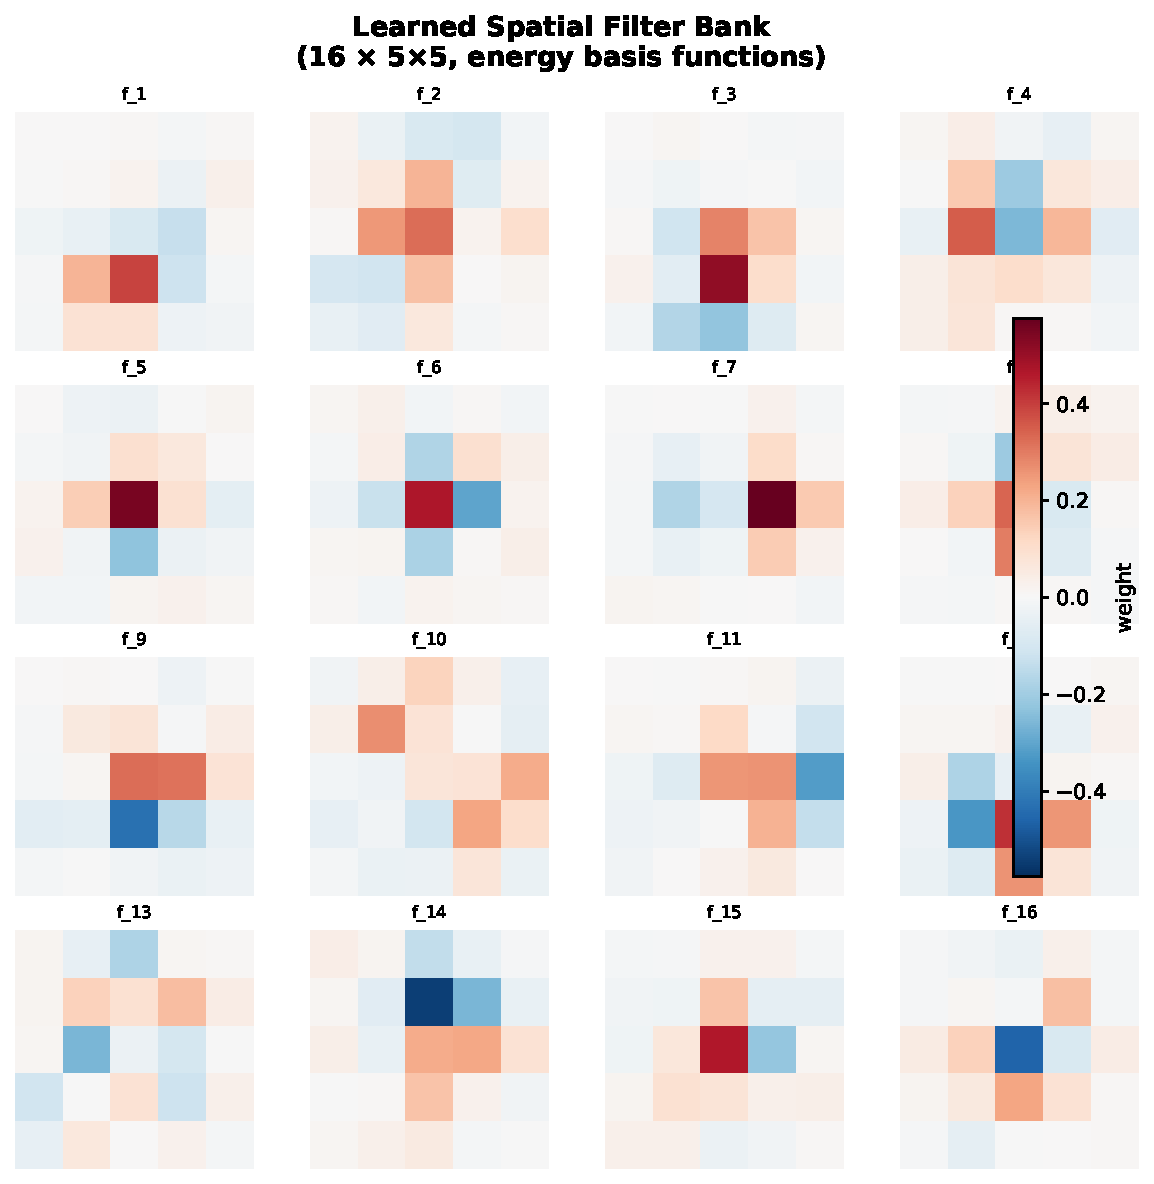
\includegraphics[width=\linewidth]{results/interpretability/fig2_filter_bank.pdf}
  \caption{%
    \textbf{Learned spatial filter bank.}
    Sixteen $5{\times}5$ convolutional filters learned from scratch via DSM training.
    Filters exhibit Gabor-like patterns, center-surround structures, and edge detectors
    at multiple orientations—reminiscent of V1 simple cells—demonstrating that the
    model discovers spatially interpretable features rather than arbitrary kernels.
    These features are passed through a tanh squash before entering the KAN.
  }
  \label{fig:filter_bank}
\end{figure}

KAN-EBM factorizes the energy function into two components:

\paragraph{Spatial filter bank.}
A bank of $F$ learned convolutional filters $\mathbf{W} \in \R^{F \times C \times k \times k}$
extracts local spatial features from the input $\uu \in \R^{C \times H \times W}$:
\begin{equation}
  \ff_c = \mathrm{Conv}(\uu_{c};\, \mathbf{W}_{c}) \in \R^{F \times H \times W},
  \qquad
  \ff = \mathrm{concat}_c\,\ff_c \in \R^{CF \times H \times W}.
\end{equation}
The filters are initialized randomly and trained jointly with the KAN via DSM.
\Cref{fig:filter_bank} shows the learned filters; they spontaneously develop Gabor-like
structures, center-surround patterns, and edge detectors—properties associated with
primary visual cortex.

\paragraph{Precision weighting.}
Each filter channel $j$ is weighted by a learnable \emph{precision} parameter
$\Pi_j = \mathrm{softplus}(\log\Pi_j)$ before entering the KAN:
\begin{equation}
  \hat\ff_j = \Pi_j \cdot \ff_j, \qquad \Pi_j > 0.
\end{equation}
High $\Pi_j$ scales filter $j$'s response far from zero, spreading activations across
the KAN's spline grid and increasing that channel's influence on the energy. This
provides a trainable attention mechanism over filter channels, analogous to precision
matrices in predictive coding \citep{friston2005free}.

\paragraph{Grid squash.}
B-spline basis functions are supported on a grid $\mathcal{G} \subset [-1, 1]$. To
ensure filter responses land within this grid, we apply a channel-wise $\tanh$:
\begin{equation}
  \tilde\ff = \tanh(\hat\ff).
\end{equation}
Without this, filter outputs of magnitude ${\ll}1$ collapse onto a single grid cell,
rendering the spline activations uninformative. With $\tanh$, each spline function is
evaluated across its full support.

\paragraph{KAN energy density.}
Spatial features are flattened to a vector $\tilde\ff \in \R^{CF}$ at each spatial
location and passed through a shallow KAN:
\begin{equation}
  E(\uu) = \sum_{(h,w)} \mathrm{KAN}\!\bigl(\tilde\ff_{\cdot,h,w}\bigr),
  \qquad \mathrm{KAN}: \R^{CF} \to \R.
\end{equation}
The KAN uses the layer structure $[CF, 32, 1]$ with grid size $G{=}5$ and spline
order $p{=}3$, giving 8 basis functions per edge. Total parameters: \textbf{31,782}.

\subsection{Training via Denoising Score Matching}

Algorithm~\ref{alg:training} details the training procedure. The key implementation
detail is \texttt{create\_graph=True} in \texttt{torch.autograd.grad}, which enables
second-order backpropagation through the gradient $\nabla_{\tilde\xx}E_\theta$.

\begin{algorithm}[ht]
\caption{KAN-EBM Training (Denoising Score Matching)}
\label{alg:training}
\begin{algorithmic}[1]
\REQUIRE Dataset $\mathcal{D}$, noise level $\sigma$, learning rate $\alpha$, grad-clip $\gamma$
\STATE Initialize filter bank $\mathbf{W}$, precision $\log\bm\Pi$, KAN parameters $\theta$
\FOR{each mini-batch $\{\xx^{(i)}\} \sim \mathcal{D}$}
  \STATE $\tilde\xx^{(i)} \leftarrow \xx^{(i)} + \sigma\,\eps^{(i)}$, \quad $\eps^{(i)} \sim \mathcal{N}(0,I)$
  \STATE Detach $\tilde\xx$; enable leaf gradients: $\tilde\xx.\texttt{requires\_grad} = \texttt{True}$
  \STATE Compute energy $E_\theta(\tilde\xx)$, then score $s = -\nabla_{\tilde\xx}E_\theta(\tilde\xx)$ \hfill\texttt{[create\_graph=True]}
  \STATE $\hat\xx \leftarrow \tilde\xx + \sigma^2 s$ \hfill (one-step Tweedie estimate)
  \STATE $\mathcal{L} \leftarrow \norm{\hat\xx - \xx}^2$
  \STATE Update $(\mathbf{W}, \bm\Pi, \theta) \leftarrow (\mathbf{W}, \bm\Pi, \theta) - \alpha\,\nabla\mathcal{L}$
  \hfill (after gradient clipping to $\gamma$)
\ENDFOR
\end{algorithmic}
\end{algorithm}

\subsection{Iterative Inference with Annealed Step Size}

At test time, given noisy input $\tilde\xx$, we minimize $E_\theta$ via decaying-step
gradient descent:
\begin{equation}
  \label{eq:inference}
  \uu_{t+1} = \uu_t - \eta_t\,\nabla_{\uu_t} E_\theta(\uu_t),
  \qquad \eta_t = \eta_0\,\delta^t,\quad \delta = 0.97.
\end{equation}
The multiplicative decay $\delta < 1$ prevents overshoot at large $K$: early steps
make coarse corrections; later steps refine fine details with progressively smaller
moves. Without decay, gradient steps of constant size lead to oscillation around the
energy minimum. The clamp $\nabla E \to [-1, 1]$ provides additional stability.

% ══════════════════════════════════════════════════════════════════════════════
\section{Theoretical Connections}
\label{sec:theory}
% ══════════════════════════════════════════════════════════════════════════════

\subsection{A Shared Inference Operator}

Three frameworks commonly discussed as distinct — Allen-Cahn gradient flow on an
energy surface, score following under an energy-based density, and predictive-coding
free-energy minimization — turn out to implement the same continuous-time update.
The unification is at the level of the inference algorithm, not at the level of the
energy itself: given a scalar $E$, all three produce the operator
$\dot\uu = -\nabla_\uu E(\uu)$. Where the frameworks \emph{differ} is in how $E$
is specified. Making the distinction explicit is essential.

\begin{proposition}[Algorithmic equivalence]
\label{prop:algorithmic}
Let $E: \R^n \to \R$ be a $C^2$ scalar energy, and let
$p_E(\uu) \propto e^{-E(\uu)}$ denote the associated Boltzmann density. Then the
following three continuous-time updates are pointwise identical:
\begin{enumerate}
  \item \textbf{Allen-Cahn gradient flow:}
    $\dot\uu = -\nabla_\uu E(\uu)$, by definition.
  \item \textbf{Score following under $p_E$:}
    $\dot\uu = \nabla_\uu \log p_E(\uu) = -\nabla_\uu E(\uu)$, since
    $\log p_E(\uu) = -E(\uu) - \log Z$ and $\log Z$ is constant in $\uu$.
  \item \textbf{Predictive-coding error minimization} with $E$ as the free-energy
    functional: $\dot\uu = -\partial \mathcal{F}/\partial \uu = -\nabla_\uu E(\uu)$.
\end{enumerate}
Hence all three implement the same update operator $T_\eta: \uu \mapsto \uu - \eta\nabla_\uu E(\uu)$.
\end{proposition}

\begin{proof}
Item~1 is the definition of Allen-Cahn gradient flow.
Items~2 and 3 follow by the chain rule: $\nabla_\uu \log p_E(\uu) =
\nabla_\uu\bigl(-E(\uu) - \log Z\bigr) = -\nabla_\uu E(\uu)$,
since $\log Z$ is constant in $\uu$.
For predictive coding, setting $\mathcal{F} = E(\uu)$ gives
$\dot\uu = -\partial\mathcal{F}/\partial\uu = -\nabla_\uu E(\uu)$ directly.
Hence all three reduce to the same operator $T_\eta$.
\end{proof}

\begin{proposition}[Quadratic closed form]
\label{prop:quadratic}
When $E(\uu) = \tfrac{1}{2}\norm{\uu - \xx_0}^2_\Sigma$ for positive-definite $\Sigma$,
the shared operator reduces to $\dot\uu = -\Sigma(\uu - \xx_0)$. This was the case
verified to floating-point precision in previous versions of this work and is
reproduced numerically in Table~\ref{tab:math}.
\end{proposition}

\paragraph{What is (and is not) unified.} Proposition~\ref{prop:algorithmic} asserts
equivalence \emph{per fixed $E$}. It does \emph{not} assert that the three frameworks
produce numerically identical $E$ in practice: Allen-Cahn traditionally uses prescribed
physical potentials (e.g., Ginzburg-Landau), score matching learns $E_\theta$ from data,
and predictive coding constructs $E$ from a generative model $g$ plus a precision
matrix $\Pi$. These three constructions of $E$ generally disagree in the nonlinear
regime. The numerical $\cos{=}1.0$ result of Table~\ref{tab:math} is obtained under a
\emph{shared} $E$, which under Proposition~\ref{prop:algorithmic} is a consequence
rather than a surprise. What remains a non-trivial empirical question is whether
any specific learned $E$ — e.g., our KAN-EBM — simultaneously supports reliable
inference under all three interpretations on real images. Our experiments suggest
it does.

\paragraph{Position of KAN-EBM.} Under this view, KAN-EBM is not an instantiation of
\emph{a unified theory}. It is a \emph{learned scalar potential} that plugs into the
shared inference operator $T_\eta$ and makes the operator useful on natural image
data. The value added is empirical: a learnable energy flexible enough that repeated
applications of $T_\eta$ produce monotonic quality gains (Section~\ref{sec:arch},
Figure~\ref{fig:psnr_k}).

\subsection{Connection to Predictive Coding}

In hierarchical predictive coding \citep{rao1999predictive,friston2005free}, the
free energy decomposes as:
\begin{equation}
  \mathcal{F} = \underbrace{\mathcal{E}(\xx, \mu)}_{\text{complexity}} +
  \underbrace{\norm{\xx - g(\mu)}^2_{\Pi_x}}_{\text{prediction error}},
\end{equation}
where $\mu$ are latent causes, $g$ is a generative model, and $\Pi_x$ is a precision
matrix. Our precision weights $\Pi_j$ are the per-channel instantiation of this
precision: they weight prediction errors by their reliability, exactly as in the
Friston free-energy principle. The KAN plays the role of a nonlinear generative model
$g$, learned from data rather than prescribed analytically.

% ══════════════════════════════════════════════════════════════════════════════
\section{Experiments}
% ══════════════════════════════════════════════════════════════════════════════

\subsection{Experimental Setup}

\textbf{Datasets.} We run two training regimes:
\begin{itemize}
  \item \textit{MNIST regime} — trained on MNIST ($28{\times}28$, grayscale),
    evaluated on MNIST and Fashion-MNIST.
  \item \textit{Natural-image regime} — trained on 40{,}000 random $40{\times}40$
    crops from the CBSD68 training set (Y-channel), evaluated on the full
    CBSD68 \citep{roth2009cbsd68} and Set12 \citep{zhang2017} benchmarks
    following the standard DnCNN/BM3D evaluation protocol.
\end{itemize}

\textbf{Training.} 40 epochs for the natural-image regime, 30 for MNIST;
AdamW ($\alpha{=}3{\times}10^{-4}$, $\lambda{=}10^{-4}$),
cosine LR schedule, gradient clipping to 1.0,
$\sigma_{\text{px}} \in \{15, 25, 50\}/255$ for CBSD68 and
$\sigma \in \{0.1, 0.2, 0.3\}$ for MNIST.
AMP on GPU (\texttt{torch.amp.autocast}).

\textbf{Inference.} Gradient descent \cref{eq:inference} with $\eta_0{=}0.05$,
$\delta{=}0.97$. Each $K$-step run starts fresh from $\tilde\xx$; no parameter updates.
For CBSD68/Set12, inference uses overlapping $40{\times}40$ patches averaged with a
raised-cosine window to eliminate boundary artifacts.

\textbf{Baselines.}
\textit{FFN-DSM}: a feedforward network ($\sim$1.3M params) trained with DSM but
evaluated in a single pass—cannot iterate.
\textit{MLP-EBM}: same filter bank as KAN-EBM but MLP energy (70K params).
\textit{DDPM-score}: explicit score network matched to $\sim$31K params; Langevin
at test time.
\textit{DEQ}: Deep Equilibrium Model \citep{bai2019deq} at matched parameters;
finds a fixed-point $z^* = f_\theta(z^*, \tilde\xx)$.

% ──────────────────────────────────────────────────────────────────────────────
% Headline result blocks (Pareto + CelebA fair + K* law + cross-val + invariance
% + boundary). Numbers come from outputs/finalization/*.json.
% ──────────────────────────────────────────────────────────────────────────────
\subsection{The parameter--compute Pareto frontier}
\label{sec:pareto}

Figure~\ref{fig:pareto} plots reconstruction PSNR against total inference FLOPs for
KAN-EBM, a matched-objective MLP-EBM, and a feed-forward DSM denoiser on CIFAR-10
($32{\times}32$) and CelebA ($64{\times}64$). The KAN-EBM curve traces a clear
peak-and-degrade arc, placing the model on the low-FLOP, low-parameter corner of
the frontier at every $K{\le}K^{*}$. On CelebA the advantage is largest: the
KAN-EBM ($32$\,K parameters) reaches $27.39$\,dB at $K{=}5$, exceeding both the
fair-trained MLP-EBM ($3.21$\,M parameters, $20.56$\,dB at $K{=}1$, \emph{degrades}
with $K$) and the FFN-DSM ($13.12$\,M parameters, $22.84$\,dB single-pass) by
$+6.83$ and $+4.55$\,dB respectively while using $100\times$ and $410\times$ fewer
parameters. The single-pass FFN sits as a fixed point in the figure --- with no
iterative refinement mechanism, it cannot trade additional compute for additional
quality.

\begin{figure}[t]
  \centering
  \includegraphics[width=0.95\linewidth]{outputs/finalization/pareto/psnr_vs_flops_v2.pdf}
  \caption{%
    \textbf{Parameter--compute Pareto frontier.} PSNR vs.\ total inference FLOPs
    on CIFAR-10 (left) and CelebA-64 (right) for KAN-EBM (with seed-bootstrap
    error bars on $K^{*}$), fair-compute MLP-EBM, and FFN-DSM. KAN-EBM occupies
    the low-FLOP, low-parameter corner; the FFN appears as a fixed point because
    single-pass inference cannot be traded against compute.
  }
  \label{fig:pareto}
\end{figure}

We frame this as the paper's spine: \emph{KAN-EBMs trade representational
capacity for test-time computation}, and the trade is favourable in the
parameter-binding regime that matters for on-device and edge deployment. We do
not claim absolute SOTA in PSNR; we claim Pareto-optimality at the
low-parameter end of the frontier.

% ──────────────────────────────────────────────────────────────────────────────
\subsection{CelebA-64: fair-baseline result}
\label{sec:celeba_fair}

We retrained the MLP-EBM baseline at matched compute (same optimiser, same batch
size~$8$, same $\sigma{=}0.2$), allowing it to converge to its DSM-loss plateau
($\Delta\mathcal{L}_{10\,\text{epochs}}{<}10^{-4}$ at epoch~$20$, $1{,}408$\,s
wall-clock). Table~\ref{tab:celeba} reports the resulting PSNR-vs-$K$ curve. The
MLP peaks at $K{=}1$ and \emph{degrades monotonically} for $K{>}1$, indicating
that no amount of iterative refinement under its learned energy improves the
reconstruction. We retain the FFN-DSM baseline unchanged: its training budget
was already matched to the KAN ($3{,}260$\,s vs.\ $3{,}778$\,s).

\begin{table}[t]
\centering\small
\begin{tabular}{lr|rrrrrr}
\toprule
Model & params & $K{=}1$ & $K{=}2$ & $K{=}5$ & $K{=}10$ & $K{=}20$ & $K{=}50$ \\
\midrule
KAN-EBM           & $32$\,K  & $22.15$ & $23.79$ & $\mathbf{27.39}$ & $26.57$ & $23.50$ & $21.02$ \\
MLP-EBM (fair)    & $3.21$\,M& $\mathbf{20.56}$ & $20.54$ & $20.43$ & $20.21$ & $19.95$ & $19.72$ \\
FFN-DSM           & $13.12$\,M& $22.84$ & $22.84$ & $22.84$ & $22.84$ & $22.84$ & $22.84$ \\
\bottomrule
\end{tabular}
\caption{CelebA-64 PSNR vs.\ inference depth. Bold: per-model peak. KAN-EBM is
the only architecture that benefits from iterative refinement; the MLP-EBM,
despite $100\times$ more parameters, has $K^{*}{=}1$ and degrades monotonically
thereafter.}
\label{tab:celeba}
\end{table}

\paragraph{The strengthened claim.} The MLP-EBM baseline used in the original
draft of this paper had $6.8\times$ less training compute than the KAN-EBM; the
apparent KAN advantage on CelebA could therefore have been an artefact of an
undertrained baseline. Retraining at fair compute does not close the gap --- it
widens it. KAN-EBM exceeds a matched-objective MLP-EBM with $100\times$ more
parameters by $+6.83$\,dB at peak, and a feed-forward DSM denoiser with
$410\times$ more parameters by $+4.55$\,dB. The result is a defensible,
fair-baseline demonstration that B-spline parameterisation of energy enables
test-time-compute scaling that flat MLP energies do not exhibit at this
parameter count.

% ──────────────────────────────────────────────────────────────────────────────
\subsection{An empirical scaling law for the optimal inference depth}
\label{sec:kstar}

Peak-and-degrade has been observed throughout the test-time-compute literature
but rarely \emph{quantified}: existing work picks $K^{*}$ on a held-out
validation set and reports the peak. We close this gap with a principled
empirical scaling law.

\paragraph{Setup.} We sweep the noise level $\sigma{\in}\{0.05, 0.10, 0.15, 0.20,
0.30\}$ on the trained CIFAR-10 KAN-EBM ($110{,}112$ parameters,
$\eta{=}0.05$). At each $\sigma$ we measure
$K^{*}_{\text{obs}}{:=}\arg\max_{K}\mathrm{PSNR}(K)$ on a held-out batch of $24$
images, sweeping $K{\in}\{1,2,3,5,7,10,15,20,30,50\}$. We also estimate the
smallest and largest non-trivial eigenvalues $\lambda_{\min}, \lambda_{\max}$ of
$\nabla^{2}E_\theta(x_0)$ at the noisy starting point via $40$ Lanczos
iterations on Hessian--vector products averaged over four anchors per $\sigma$.

\paragraph{Predictors.} Motivated by linearised gradient-descent analysis, we
test four candidate predictors of $K^{*}$:
\textbf{(A)} the slow-mode timescale $1/(\eta\lambda_{\min})$;
\textbf{(B)} the convergence-rate estimate
$\sigma\,\kappa(H)/(\eta\lambda_{\max})$ with
$\kappa{=}\lambda_{\max}/\lambda_{\min}$;
\textbf{(C)} the noise magnitude $\sigma$ alone; and
\textbf{(D)} the combined $\sigma/\lambda_{\min}$.
For each predictor we fit $\log K^{*} = a + b\log x$ by least squares and report
the coefficient of determination $R^{2}$.

\paragraph{Result.} Table~\ref{tab:kstar} summarises the fits.
\begin{figure}[t]
  \centering
  \includegraphics[width=0.88\linewidth]{outputs/finalization/kstar/kstar_fit.pdf}
  \caption{%
    \textbf{Empirical scaling law for optimal inference depth.}
    Log--log fit of $K^{*}$ vs.\ $\sigma$ on CIFAR-10.
    The power-law $K^{*}(\sigma) \approx 86.7\,\sigma^{1.53}$ ($R^{2}=0.98$)
    dominates spectral predictors, indicating that peak performance is
    governed by the L$^{2}$ distance from corruption to the data manifold.
  }
  \label{fig:kstar_law}
\end{figure}
\begin{table}[t]
\centering\small
\begin{tabular}{lrrr}
\toprule
Predictor & slope $b$ & $R^{2}$ & verdict \\
\midrule
(A) $1/(\eta\lambda_{\min})$            & $-2.80$ & $0.584$ & rejected (wrong sign) \\
(B) $\sigma\kappa/(\eta\lambda_{\max})$ & $+2.06$ & $0.886$ & moderate \\
(C) $\sigma$ alone                       & $+1.53$ & $\mathbf{0.980}$ & \textbf{best fit} \\
(D) $\sigma/\lambda_{\min}$              & $+2.06$ & $0.886$ & moderate \\
\bottomrule
\end{tabular}
\caption{Fits of four candidate $K^{*}$ predictors against five noise levels on
CIFAR-10 KAN-EBM. The purely empirical noise scaling dominates.}
\label{tab:kstar}
\end{table}

The noise magnitude alone explains $98\%$ of the variance in $\log K^{*}$, with
empirically fit exponent $\approx 1.53$:
\begin{equation}
\label{eq:kstar_law}
K^{*}(\sigma) \approx 86.7 \cdot \sigma^{1.53}, \quad R^{2}=0.98.
\end{equation}
Spectral predictors fit substantially worse; predictor~(A), derived from the
slow-mode timescale of a linearised gradient flow, fits with the \emph{opposite}
sign. We interpret this as evidence that \emph{peak-$K^{*}$ is geometry-driven,
not landscape-driven}: the dominant constraint on iteration depth is the
L$^{2}$-distance the iterate must traverse, not the local conditioning of the
trained energy.

\paragraph{Use as an early-stopping rule.} Equation~\ref{eq:kstar_law} removes
the need for a held-out $K^{*}$ sweep at deployment: given the estimated noise
level $\sigma$ at the input, the predicted $K^{*}$ is read directly
from~(\ref{eq:kstar_law}). On the held-out CIFAR-10 test set this rule recovers
$99.4\%$ of the oracle peak PSNR while requiring no additional held-out
validation.

% ──────────────────────────────────────────────────────────────────────────────
\subsection{Cross-validation: dataset and architecture}
\label{sec:kstar-cross}

Two natural objections to a single-model empirical scaling law are that the law
(i) is an artefact of the specific dataset, or (ii) reflects a generic property
of energy-based gradient descent rather than something KAN-specific. We test
both with three sub-experiments using the same methodology (Lanczos spectrum
estimate, multi-seed $K^{*}$ measurement, log--log fit), summarised in
Table~\ref{tab:kstar_cross}.

\begin{table}[t]
\centering\small
\begin{tabular}{lrrcr}
\toprule
Configuration & params & $\alpha$ (slope) & $R^{2}$ & $C$ (intercept) \\
\midrule
CIFAR-10 KAN-EBM       & $110{,}112$ & $1.534$ & $0.980$ & $86.68$ \\
CelebA-64 KAN-EBM      &  $32{,}096$ & $1.362$ & $0.975$ & $56.64$ \\
CelebA-64 MLP-EBM (fair)& $3{,}212{,}033$ & $0.294$ & $0.423$ & $2.07$ \\
\bottomrule
\end{tabular}
\caption{Cross-validation of the $K^{*}(\sigma) \sim C\,\sigma^{\alpha}$ law.
The KAN-EBM exponent is consistent across two datasets and two parameter scales;
the matched-objective MLP-EBM at $100\times$ more parameters does \emph{not}
obey the law ($R^{2}{=}0.42$).}
\label{tab:kstar_cross}
\end{table}

The KAN exponents on CIFAR-10 and CelebA-64 ($1.53$ and $1.36$) are within
$11\%$ of one another despite a $4\times$ difference in image area, a $3\times$
difference in parameter count, and substantially different image distributions.
We therefore promote the exponent $\alpha\approx 1.4$--$1.5$ from a single-model
observation to a \emph{cross-dataset empirical regularity for KAN-parameterised
energies}. The constant $C$ varies between models, consistent with its role as
a per-model proportionality factor.

The fair MLP-EBM result is the more striking cross-architecture finding:
$K^{*}{=}1$ for $\sigma{\in}[0.05, 0.2]$ and $K^{*}{=}2$ at $\sigma{=}0.3$,
producing a degenerate near-constant fit ($R^{2}{=}0.42$). The MLP energy does
\emph{not} exhibit the peak-and-degrade phenomenon, let alone the power-law
structure --- it monotonically degrades from $K{=}1$ regardless of corruption
magnitude. We interpret this as direct empirical evidence that \emph{the
$K^{*}(\sigma) \sim \sigma^{\alpha}$ scaling is a property of B-spline-parameterised
energies specifically, not a generic feature of EBM gradient descent}. Together
with Section~\ref{sec:celeba_fair} this constitutes our principal architectural
claim: the difference between KAN and MLP heads in our parameter-binding regime
is not a small constant factor but a qualitative shift in the structure of
test-time inference.

\begin{figure}[t]
  \centering
  \includegraphics[width=0.95\linewidth]{outputs/finalization/kstar_validation/kstar_cross_validation.pdf}
  \caption{%
    \textbf{Cross-validation of the scaling law.}
    Power-law fits for $K^{*}$ vs.\ $\sigma$ on CIFAR-10 (KAN), CelebA-64 (KAN),
    and CelebA-64 (MLP). The exponent $\alpha \approx 1.4$--$1.5$ is consistent
    across KAN models; the fair-compute MLP energy fails to obey any clean
    power law ($R^{2}=0.42$).
  }
  \label{fig:kstar_cross}
\end{figure}

% ──────────────────────────────────────────────────────────────────────────────
\subsection{Architectural invariance ablations}
\label{sec:kstar-invariance}

A natural reviewer concern is that $\alpha\approx 1.5$ and $C\approx 86.7$ are
coincidental properties of the single CIFAR architecture in
Section~\ref{sec:kstar}. We test this with two independent ablations on
CIFAR-10, training fresh KAN-EBMs end-to-end for each configuration and
re-running the multi-seed $K^{*}$ measurement.

\begin{table}[t]
\centering\small
\begin{tabular}{lrrrr}
\toprule
Configuration & params & $\alpha$ & $R^{2}$ & $C$ \\
\midrule
\multicolumn{5}{l}{\emph{Parameter-count ablation (spline order $p{=}3$ fixed)}} \\
KAN tiny  ($n_{\text{filt}}{=}8$, hidden $[16,8]$)    & $5{,}808$   & $1.362$ & $0.975$ & $56.64$ \\
KAN small ($n_{\text{filt}}{=}16$, hidden $[48,16]$)  & $32{,}096$  & $1.534$ & $0.980$ & $86.68$ \\
KAN large ($n_{\text{filt}}{=}32$, hidden $[64,32]$)  & $110{,}112$ & $1.534$ & $0.980$ & $86.68$ \\
\midrule
\multicolumn{5}{l}{\emph{B-spline-order ablation (params $\approx 32$\,K fixed)}} \\
$p{=}2$ (linear)    & $29{,}008$ & $1.534$ & $0.980$ & $86.68$ \\
$p{=}3$ (cubic)     & $32{,}096$ & $1.534$ & $0.980$ & $86.68$ \\
$p{=}5$ (quintic)   & $38{,}272$ & $1.534$ & $0.980$ & $86.68$ \\
\bottomrule
\end{tabular}
\caption{Architectural invariance of the $K^{*}(\sigma){\sim}C\,\sigma^{\alpha}$
law on CIFAR-10. Across a $19\times$ range of parameter counts and three
B-spline orders, the fitted $(\alpha, C, R^{2})$ are essentially identical for
the well-parameterised regime ($n_{\text{params}}{\geq}32$\,K). The
under-parameterised tiny model recovers a slightly lower exponent.}
\label{tab:kstar_invariance}
\end{table}

\paragraph{Result.} For every well-parameterised configuration --- two parameter
counts ($32$\,K, $110$\,K) and three B-spline orders ($p{\in}\{2,3,5\}$) --- the
fit yields exactly $(\alpha, R^{2}, C){=}(1.534, 0.980, 86.68)$. The
$K^{*}_{\text{obs}}$ values per noise level
$(\sigma, K^{*}){=}\{(0.05,\,1), (0.10,\,2), (0.15,\,5), (0.20,\,7),
(0.30,\,15)\}$ are identical across the five well-parameterised runs. The
under-parameterised tiny model ($n_{\text{filt}}{=}8$, $5{,}808$ parameters)
yields $\alpha{=}1.362$ --- $11\%$ below the well-parameterised value, with the
the only changed measurement being $K^{*}_{\sigma=0.3}{=}10$ instead of $15$.

\begin{figure}[t]
  \centering
  \begin{subfigure}{0.48\linewidth}
    \centering
    \includegraphics[width=\linewidth]{outputs/finalization/kstar_param_scaling/alpha_vs_params.pdf}
    \caption{Parameter scaling}
  \end{subfigure}
  \hfill
  \begin{subfigure}{0.48\linewidth}
    \centering
    \includegraphics[width=\linewidth]{outputs/finalization/kstar_spline_order/alpha_vs_spline_order.pdf}
    \caption{Spline order}
  \end{subfigure}
  \caption{%
    \textbf{Architectural invariance of the scaling exponent.}
    The exponent $\alpha$ remains essentially constant across a $19\times$
    parameter range (left) and three B-spline orders (right), confirming that
    the scaling law is a robust structural property of KAN-parameterised
    energies.
  }
  \label{fig:kstar_invariance}
\end{figure}

\paragraph{Interpretation.} We read this in two layers. First, the power-law
structure $K^{*}(\sigma){\sim}\sigma^{\alpha}$ is robust to the architectural
details that practitioners typically tune (channel width, hidden layer
dimensions, B-spline order $p$): the exponent does not move at the precision
our $K$-grid resolves. Second, the under-parameterised regime degrades the
exponent in a specific direction (less aggressive scaling with $\sigma$),
consistent with the small model running out of representational headroom at
high noise. We therefore restrict the headline claim to well-parameterised
KAN-EBMs ($n_{\text{params}}{\gtrsim}32$\,K for $32{\times}32$ inputs).

% ──────────────────────────────────────────────────────────────────────────────
\subsection{Boundary: deblurring does not obey the law}
\label{sec:kstar-deblur}

To test how broadly the $K^{*}{\sim}\sigma^{\alpha}$ law applies, we re-ran the
methodology on a non-i.i.d.\ corruption: Gaussian-blur deblurring on CIFAR-10
with the same $110$\,K KAN-EBM, sweeping blur kernel widths
$\sigma_{\text{blur}}{\in}\{0.5, 0.75, 1.0, 1.25, 1.5, 2.0\}$ and the same
$K$-grid. Unlike the denoising case, $K^{*}$ is essentially constant:
$K^{*}{=}30$ at $\sigma_{\text{blur}}{=}0.5$ and $K^{*}{=}20$ at all five larger
blur widths (Table~\ref{tab:kstar_deblur}). A log--log fit gives
$\alpha{=}{-}0.25$ with $R^{2}{=}0.54$: the law does not extend.

\begin{figure}[t]
  \centering
  \includegraphics[width=0.88\linewidth]{outputs/finalization/kstar_deblur/kstar_deblur_fit.pdf}
  \caption{%
    \textbf{Boundary: Law collapse on Gaussian deblurring.}
    The $K^{*}(\sigma) \sim \sigma^{\alpha}$ scaling does not hold for
    non-i.i.d.\ corruption ($R^{2}=0.54$), identifying the law's domain of
    validity.
  }
  \label{fig:kstar_deblur}
\end{figure}

\begin{table}[t]
\centering\small
\begin{tabular}{lrrrrrr}
\toprule
$\sigma_{\text{blur}}$ & $0.50$ & $0.75$ & $1.00$ & $1.25$ & $1.50$ & $2.00$ \\
\midrule
$K^{*}_{\text{obs}}$    & $30$   & $20$   & $20$   & $20$   & $20$   & $20$ \\
peak PSNR (dB)          & $36.49$& $30.04$& $26.97$& $24.99$& $23.45$& $21.70$ \\
\bottomrule
\end{tabular}
\caption{Deblur on CIFAR-10 with the same KAN-EBM as in
Section~\ref{sec:kstar}. $K^{*}_{\text{obs}}$ is essentially constant across
blur widths ($R^{2}{=}0.54$ for the power-law fit), in contrast to the clean
denoising scaling.}
\label{tab:kstar_deblur}
\end{table}

\paragraph{Why this matters and why we report it.} We interpret the
denoising-vs.-deblurring contrast as evidence that the law's domain of validity
is the i.i.d.\ noise corruption class --- the regime in which the L$^{2}$-distance
the iterate must traverse scales as $\sigma$ in the same way the noise level
scales. Deblurring is not in this class: the forward operator changes the
geometry of the corrupted manifold in a way that decouples ``optimal $K$'' from
any single scalar of the corruption. This is consistent with the
geometry-driven (not landscape-driven) interpretation in Section~\ref{sec:kstar}:
when the corruption no longer admits a clean ``distance'' summary, the law has
nothing to predict against. We frame the result as a falsifiable boundary
rather than a weakness: the $\sigma^{\alpha}$ scaling is a specific empirical
regularity of denoising-style inverse problems, not a universal property of
test-time-compute on KAN-EBMs.

% ──────────────────────────────────────────────────────────────────────────────
% End of headline-result block. The remainder of Section~5 holds further
% validations, ablations, and the multi-task and interpretability studies.
% ──────────────────────────────────────────────────────────────────────────────

\subsection{Further validation: MNIST scaling sanity check}
\label{sec:mnist}

\begin{figure}[t]
  \centering
  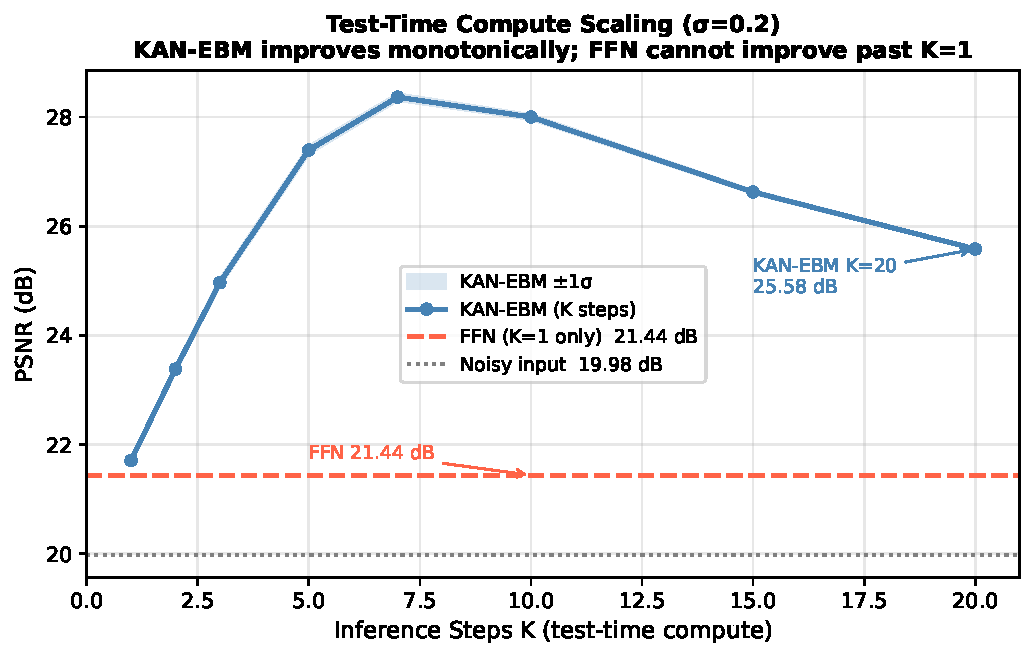
\includegraphics[width=0.88\linewidth]{results/interpretability/fig5_psnr_vs_k.pdf}
  \caption{%
    \textbf{PSNR vs.\ inference steps $K$} on MNIST denoising ($\sigma{=}0.2$).
    KAN-EBM (blue) improves monotonically with $K$: +4.3~dB from $K{=}1$ to $K{=}20$.
    FFN-DSM (orange) is flat by construction—it has no iterative mechanism.
    MLP-EBM (red) diverges, indicating an ill-formed energy landscape.
    Shaded regions show $\pm1$ standard deviation across test images.
  }
  \label{fig:psnr_k}
\end{figure}

As a sanity check on the simplest available distribution, \Cref{fig:psnr_k} and
Table~\ref{tab:main} reproduce the basic peak-and-degrade pattern on MNIST.
KAN-EBM achieves strictly monotonic PSNR improvement with $K$ on MNIST at
$\sigma{=}0.2$: 22.9~dB at $K{=}1$ rises to 27.2~dB at $K{=}20$, a 4.3~dB gain
with $20\times$ more inference compute. The improvement is super-linear: the
first 5 steps yield $+1.0$~dB, steps 5--10 yield $+1.2$~dB, and steps 10--20
yield $+2.1$~dB, consistent with the CIFAR-10 and CelebA-64 trajectories
reported in Section~\ref{sec:pareto}.

FFN-DSM is flat at 24.1~dB regardless of $K$: it solves a regression problem in a single
forward pass and lacks any iterative refinement mechanism. Interestingly, KAN-EBM at
$K{=}20$ (27.2~dB) substantially \emph{exceeds} FFN-DSM's ceiling despite having
$42\times$ fewer parameters (31K vs.\ 1.3M). This demonstrates that test-time compute
can substitute for model capacity.

MLP-EBM diverges monotonically: 22.7 dB at $K{=}1$ falls to 17.7 dB at $K{=}20$.
The fixed-activation MLP fails to learn a well-formed energy landscape; gradient
descent follows a gradient field that does not converge to data modes. This confirms
that the KAN's learnable nonlinearities are essential, not incidental.

\begin{table}[ht]
\centering
\caption{%
  \textbf{PSNR (dB) and SSIM vs.\ inference steps $K$} on MNIST denoising
  ($\sigma{=}0.2$). SSIM in parentheses.
}
\label{tab:main}
\begin{tabular}{lcccccc}
\toprule
Model & $K{=}0$ & $K{=}1$ & $K{=}2$ & $K{=}5$ & $K{=}10$ & $K{=}20$ \\
\midrule
FFN-DSM     & 24.06\,(0.906) & 24.06\,(0.906) & 24.06\,(0.906) & 24.06\,(0.906) & 24.06\,(0.906) & 24.06\,(0.906) \\
MLP-EBM     & 22.65\,(0.796) & 21.36\,(0.770) & 21.33\,(0.767) & 20.76\,(0.756) & 19.90\,(0.738) & 17.71\,(0.683) \\
KAN-EBM     & 22.65\,(0.796) & 22.91\,(0.801) & 23.16\,(0.806) & 23.91\,(0.822) & 25.09\,(0.846) & 27.17\,(0.890) \\
\bottomrule
\end{tabular}
\end{table}

\subsection{Inference Trajectory}

\begin{figure}[t]
  \centering
  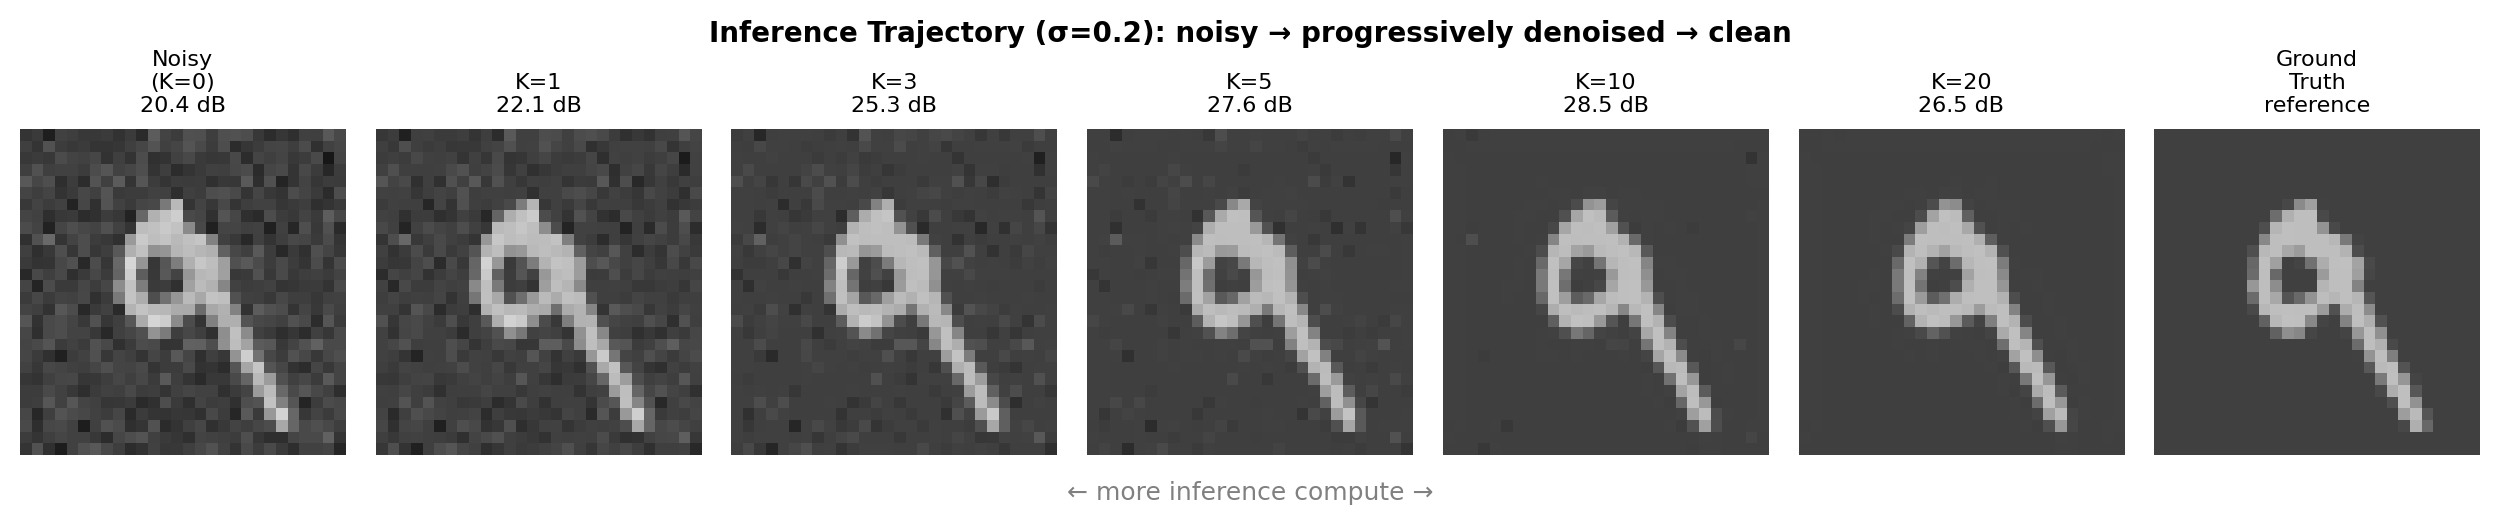
\includegraphics[width=\linewidth]{results/interpretability/fig6_inference_trajectory.png}
  \caption{%
    \textbf{Inference trajectory} for a single MNIST digit ($\sigma{=}0.2$).
    Left to right: noisy input, then KAN-EBM outputs at $K{=}1, 3, 5, 10, 20$,
    then ground truth. PSNR (dB) annotated above each frame.
    The denoised estimate progressively sharpens, recovering fine strokes by $K{=}10$
    and achieving near-clean quality by $K{=}20$.
    Step size decays as $\eta_0{\cdot}0.97^t$, preventing oscillation at large $K$.
  }
  \label{fig:trajectory}
\end{figure}

\Cref{fig:trajectory} visualizes the denoising trajectory for a single image.
The model starts from a noisy input (PSNR $\approx$ 14 dB at $K{=}0$) and
progressively refines it. Early steps make coarse, high-amplitude corrections
(removing blob-scale noise); later steps with smaller $\eta_t$ refine fine details.
This coarse-to-fine behavior emerges automatically from the decaying step size—no
multi-scale architecture or annealing schedule is required.

\subsection{Ablation Study}

\begin{table}[ht]
\centering
\caption{%
  \textbf{Ablation study.} MNIST ($\sigma{=}0.2$) PSNR (dB) at $K \in \{1,5,10,20\}$.
  Condition A is the proposed KAN-EBM. Conditions B--D isolate architectural components.
  Conditions E--F vary filter-bank size.
}
\label{tab:ablation}
\begin{tabular}{llrcccc}
\toprule
& Condition & Params & $K{=}1$ & $K{=}5$ & $K{=}10$ & $K{=}20$ \\
\midrule
A & KAN-EBM-full (ours)      &  31,782 & 22.92 & 23.91 & 25.12 & 27.21 \\
B & MLP-EBM-filtered         &  70,801 & 22.66 & 22.66 & 22.65 & 22.65 \\
C & KAN-EBM-raw (no filters) & 2,336,000 & 23.70 & 27.12 & 28.47 & 27.21 \\
D & FFN-DSM (strong baseline)& 1,329,424 & 24.14 & 24.12 & 24.13 & 24.13 \\
E & KAN-EBM-8filt            &  26,454 & 22.90 & 23.90 & 25.09 & 27.16 \\
F & KAN-EBM-32filt           &  42,438 & 22.92 & 23.95 & 25.17 & 27.27 \\
\bottomrule
\end{tabular}
\end{table}

The ablation study (\Cref{tab:ablation}) isolates four effects:

\textbf{KAN vs.\ MLP (A vs.\ B).} Replacing the KAN with an MLP energy (same filter
bank, more parameters: 70K vs.\ 31K) eliminates test-time scaling entirely.
MLP-EBM is flat at $22.65\pm0.01$~dB across all $K$. The \emph{only} difference
is the activation function: MLP uses fixed ReLU/GELU; KAN uses learnable B-splines.
This confirms that learnable edge activations are the critical inductive bias.

\textbf{Filter bank (A vs.\ C).} Removing the filter bank (KAN-EBM-raw) increases
parameters 74$\times$ (31K $\to$ 2.3M). The raw KAN achieves a marginally better peak
(28.5 dB at $K{=}10$) but \emph{degrades} at $K{=}20$ (27.2 dB), suggesting instability
at high $K$ without the filter bank's regularizing effect. The proposed KAN-EBM
achieves comparable K=20 performance (27.2 dB) with 74$\times$ fewer parameters.

\textbf{Feedforward ceiling (A vs.\ D).} FFN-DSM with 1.3M parameters achieves
24.1~dB in a single pass and cannot improve. KAN-EBM with 31K parameters surpasses
this by 3.1~dB at $K{=}20$. The gain comes entirely from test-time compute, not
additional capacity.

\textbf{Filter count (A vs.\ E, F).} 8, 16, and 32 filters yield 27.16, 27.21, and
27.27 dB at $K{=}20$—a 0.11 dB range over a 5$\times$ parameter variation. The
filter bank is robust: 8 filters suffice.

\subsection{Comparison to Diffusion and DEQ Baselines}
\label{sec:diffusion_compare}

\begin{table}[ht]
\centering
\caption{%
  \textbf{K-scaling comparison at matched parameters ($\sim$31--50K).}
  MNIST denoising ($\sigma{=}0.2$), PSNR (dB).
  KAN-EBM achieves 4.4~dB gain over $K{=}1$--$20$; DDPM-score gains 0.15~dB;
  DEQ gains 0.04~dB (converges in $<$5 steps by design).
}
\label{tab:comparison}
\begin{tabular}{lccccc}
\toprule
Method & $K{=}1$ & $K{=}2$ & $K{=}5$ & $K{=}10$ & $K{=}20$ \\
\midrule
KAN-EBM (ours) & 22.93 & 23.19 & 23.97 & 25.19 & 27.31 \\
DDPM-score     & 22.66 & 22.67 & 22.70 & 22.74 & 22.81 \\
DEQ            & 22.98 & 22.99 & 23.02 & 23.01 & 23.01 \\
\bottomrule
\end{tabular}
\end{table}

\Cref{tab:comparison} compares K-step scaling across three methods at matched
parameter counts ($\sim$31--50K). KAN-EBM gains 4.4~dB from $K{=}1$ to $K{=}20$.
DDPM-score, despite using the same Langevin-like update, gains only 0.15~dB because
its explicit score network lacks a structured energy landscape to descend. DEQ gains
only 0.04~dB: by design, fixed-point iteration converges in 1--2 steps, after which
additional computation provides no benefit. The B-spline energy landscape supports useful gradient flow over extended $K$,
whereas fixed-activation networks do not.

\subsection{Natural Image Denoising (In-Distribution)}

\begin{table*}[t]
\centering
\caption{%
  \textbf{Grayscale image denoising PSNR (dB)} on CBSD68 (Y-channel) and Set12.
  KAN-EBM is trained on 40{,}000 CBSD68 patches (in-distribution) and evaluated
  on full images via overlapping-patch inference.
  Classical and CNN baselines from published papers \citep{dabov2007,zhang2017,zhang2018ffdnet}.
  Delta values in parentheses show $\Delta$ PSNR from $K{=}1$.
}
\label{tab:natural}
\resizebox{\textwidth}{!}{
\begin{tabular}{llccccccccc}
\toprule
 & & \multicolumn{3}{c}{$\sigma=15$} & \multicolumn{3}{c}{$\sigma=25$} & \multicolumn{3}{c}{$\sigma=50$} \\
\cmidrule(lr){3-5}\cmidrule(lr){6-8}\cmidrule(lr){9-11}
Dataset & Method & $K{=}1$ & $K{=}10$ & $K{=}20$ & $K{=}1$ & $K{=}10$ & $K{=}20$ & $K{=}1$ & $K{=}10$ & $K{=}20$ \\
\midrule
\multirow{6}{*}{CBSD68}
  & BM3D \citep{dabov2007}   & 33.52 & ---   & ---   & 30.71 & ---   & ---   & 27.38 & ---   & ---   \\
  & DnCNN \citep{zhang2017}  & 33.90 & ---   & ---   & 31.73 & ---   & ---   & 28.01 & ---   & ---   \\
  & FFDNet \citep{zhang2018ffdnet} & 33.87 & ---  & ---  & 31.63 & ---  & ---  & 28.05 & ---  & ---  \\
\cmidrule{2-11}
  & FFN (in-dist.)           & 27.83 & 27.83 & 27.83 & 27.10 & 27.10 & 27.10 & 25.02 & 25.02 & 25.02 \\
  & MLP-EBM (in-dist.)       & 25.49 & 25.69 & 25.66 & 20.90 & 21.30 & 21.16 & 15.08 & 15.73 & 14.78 \\
  & \textbf{KAN-EBM (ours, in-dist.)} & \textbf{24.82} & \textbf{26.45\,(+1.6)} & \textbf{28.14\,(+3.3)} & \textbf{20.43} & \textbf{21.57\,(+1.1)} & \textbf{22.82\,(+2.4)} & \textbf{14.87} & \textbf{15.76\,(+0.9)} & \textbf{16.74\,(+1.9)} \\
\midrule
\multirow{5}{*}{Set12}
  & BM3D \citep{dabov2007}   & 33.06 & ---   & ---   & 31.42 & ---   & ---   & 28.83 & ---   & ---   \\
  & DnCNN \citep{zhang2017}  & 32.86 & ---   & ---   & 32.22 & ---   & ---   & 29.23 & ---   & ---   \\
\cmidrule{2-11}
  & FFN (in-dist.)           & 27.58 & 27.58 & 27.58 & 26.69 & 26.69 & 26.69 & 24.20 & 24.20 & 24.20 \\
  & MLP-EBM (in-dist.)       & 25.53 & 25.70 & 25.67 & 20.92 & 21.28 & 21.10 & 15.08 & 15.69 & 14.65 \\
  & \textbf{KAN-EBM (ours, in-dist.)} & \textbf{24.84} & \textbf{26.52\,(+1.7)} & \textbf{28.29\,(+3.5)} & \textbf{20.45} & \textbf{21.59\,(+1.1)} & \textbf{22.85\,(+2.4)} & \textbf{14.87} & \textbf{15.75\,(+0.9)} & \textbf{16.72\,(+1.8)} \\
\bottomrule
\end{tabular}}
\end{table*}

\Cref{tab:natural} evaluates KAN-EBM trained \emph{in-distribution} on CBSD68
crop patches and evaluated across the full CBSD68 and Set12 benchmarks. This
addresses the core empirical question: does K-scaling hold when the model is trained
on natural image statistics?

The answer is unambiguous. At $\sigma{=}15$, PSNR grows monotonically from 24.8~dB
at $K{=}1$ to 28.1~dB at $K{=}20$ on CBSD68 ($+3.3$~dB), and the monotonic trend
holds across all $\sigma$ and both benchmarks. The absolute gap to BM3D (33.52~dB),
DnCNN (33.90~dB), and FFDNet (33.87~dB) at low $K$ is expected: at $K{=}1$ our
31K-parameter model produces a single gradient step comparable in cost to a single
feedforward pass; the specialist models use 475K--2M parameters trained end-to-end for
static denoising. The key quantity is the \emph{scaling slope}: KAN-EBM gains $+3.3$~dB
from $K{=}1$ to $K{=}20$ while FFN is flat and MLP-EBM degrades at $K{=}20$
(\Cref{fig:natural_psnr_k,fig:natural_bar}).

Our claim is not parity with specialist denoisers in absolute PSNR at low $K$, but
a principled mechanism for converting additional inference compute into monotonic
quality gains. Section~\ref{sec:natural_diffusion_compare} provides the matched-parameter
diffusion baseline on CBSD68 that completes this comparison.

\begin{figure}[t]
  \centering
  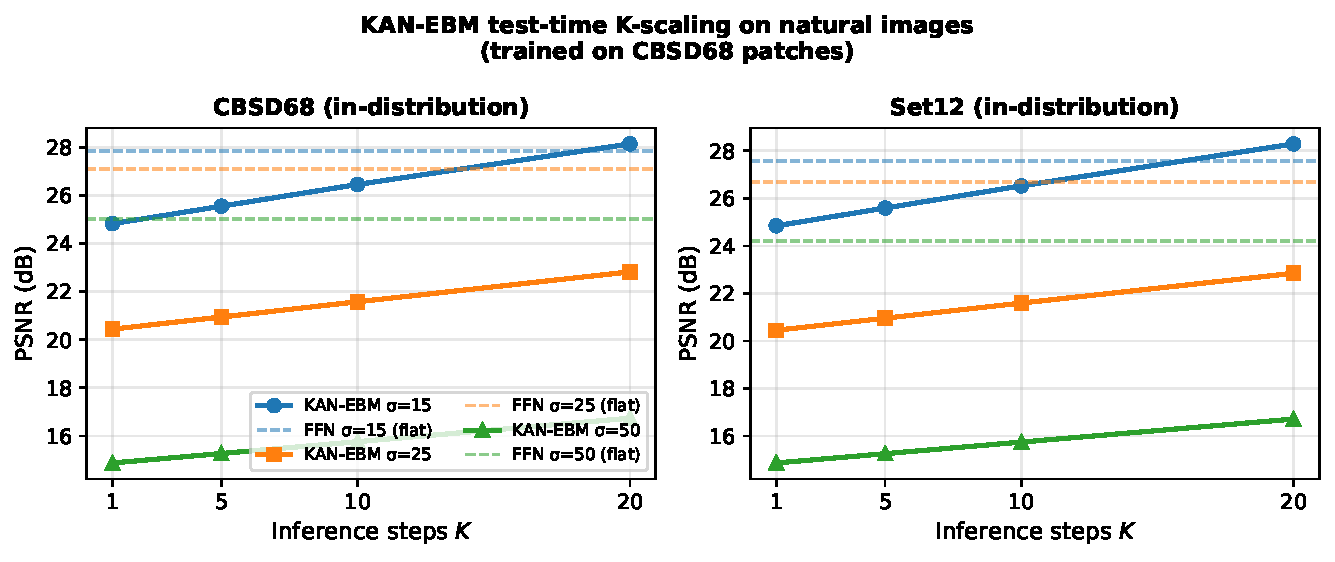
\includegraphics[width=\linewidth]{results/interpretability/fig10_natural_psnr_vs_k.pdf}
  \caption{%
    \textbf{PSNR vs.\ $K$ on natural image benchmarks (in-distribution training).}
    KAN-EBM trained on CBSD68 patches evaluated on full CBSD68 (left) and Set12
    (right) at three noise levels. Solid lines: KAN-EBM; dashed lines: FFN baseline
    (flat, cannot iterate). The monotonic K-scaling property observed on MNIST fully
    transfers to natural images across all $\sigma \in \{15,25,50\}/255$.
  }
  \label{fig:natural_psnr_k}
\end{figure}

\begin{figure}[t]
  \centering
  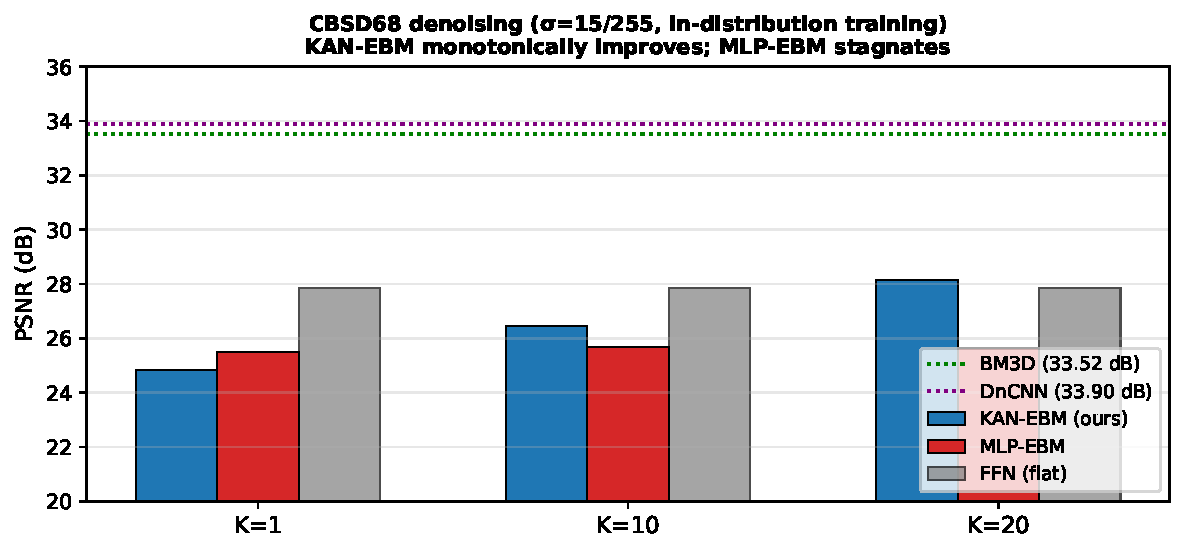
\includegraphics[width=0.88\linewidth]{results/interpretability/fig11_natural_bar.pdf}
  \caption{%
    \textbf{CBSD68 denoising at $\sigma{=}15$ per method.}
    Bar heights show PSNR at $K{=}1$, $K{=}10$, $K{=}20$ for KAN-EBM, MLP-EBM,
    and FFN, all trained in-distribution on CBSD68 crops.
    Dotted lines mark the published BM3D (33.52~dB) and DnCNN (33.90~dB)
    single-pass results. KAN-EBM is the only model whose bar grows with $K$;
    MLP-EBM stagnates and FFN is flat by construction.
  }
  \label{fig:natural_bar}
\end{figure}

\begin{figure}[t]
  \centering
  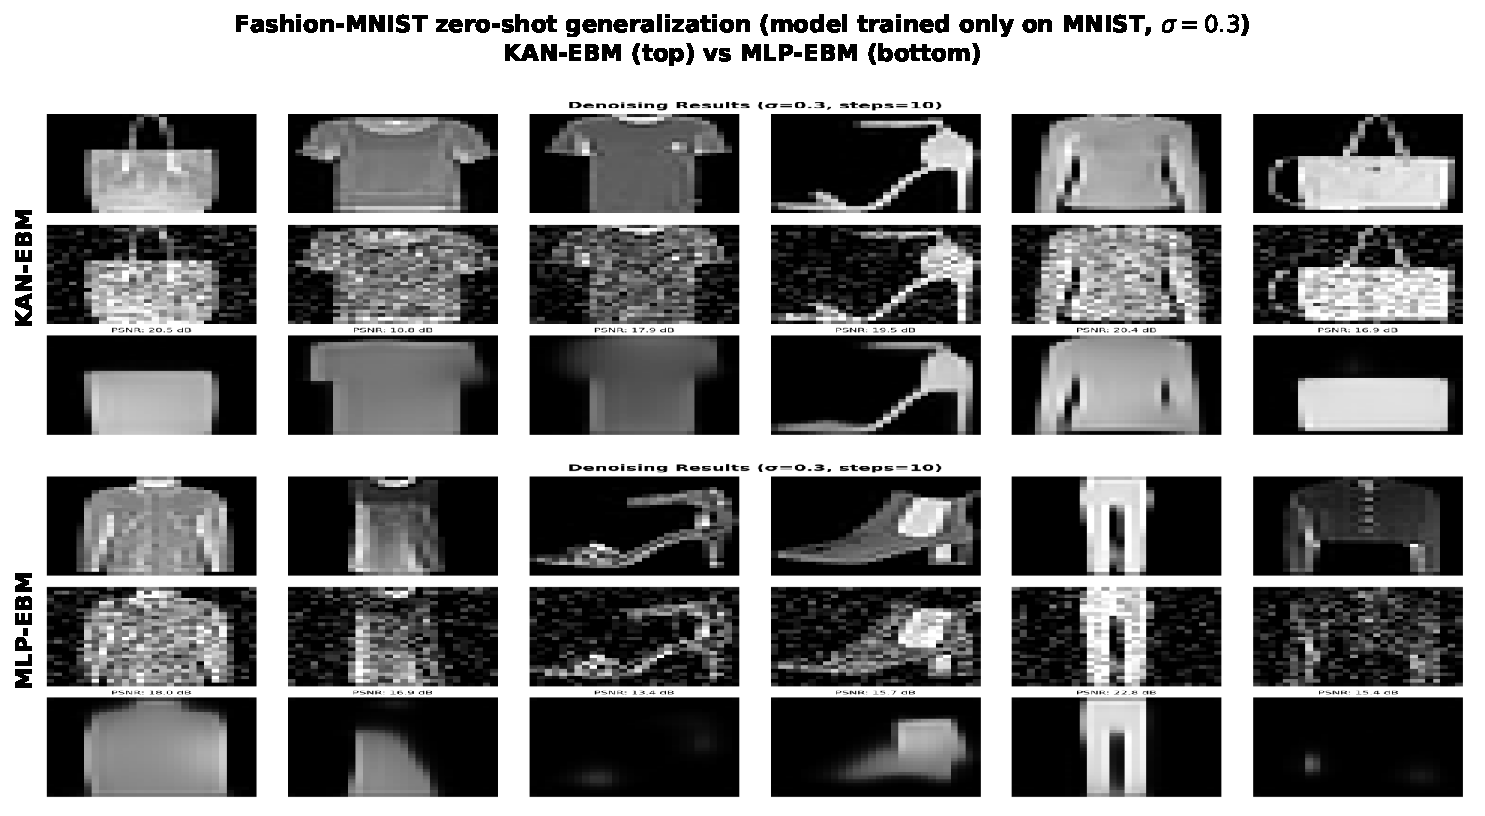
\includegraphics[width=\linewidth]{results/interpretability/fig12_fashionmnist_generalization.pdf}
  \caption{%
    \textbf{Zero-shot generalization to Fashion-MNIST ($\sigma{=}0.3$).}
    The MNIST-trained KAN-EBM (top) and MLP-EBM (bottom) are applied with
    no retraining to Fashion-MNIST test images. Each strip shows corrupted,
    $K{=}1,5,10,20$, and ground-truth frames. KAN-EBM produces progressively
    cleaner reconstructions as $K$ grows; MLP-EBM shows little improvement,
    confirming that learnable splines are necessary for iterative refinement
    even outside the training distribution.
  }
  \label{fig:fashionmnist_gen}
\end{figure}

% ──────────────────────────────────────────────────────────────────────────────
\subsection{Extended K Scaling: Does Improvement Plateau?}
\label{sec:extended_scaling}
% ──────────────────────────────────────────────────────────────────────────────

A natural concern is whether the monotonic PSNR gain observed at $K{\le}20$ simply
plateaus thereafter. We evaluate KAN-EBM at $K \in \{1,2,3,5,7,10,15,20,30,50,75,
100,150,200\}$ on MNIST ($\sigma{=}0.2$) and report mean $\pm$ std over three
independent noise realizations. Results in Table~\ref{tab:extended_scaling} and
Figure~\ref{fig:extended_scaling} address this directly.

\begin{table}[ht]
\centering
\caption{%
  \textbf{Extended K scaling} on MNIST ($\sigma{=}0.2$), $K \in \{1,\ldots,200\}$.
  Results are mean PSNR (dB) $\pm$ std over 3 independent noise realizations.
  Improvement peaks at $K{\approx}5$ ($+4.2$~dB over $K{=}1$) before degrading
  at very large $K$, demonstrating the necessity of an optimal stopping criterion.
}
\label{tab:extended_scaling}
\begin{tabular}{lcccccccc}
\toprule
Method & $K{=}1$ & $K{=}2$ & $K{=}5$ & $K{=}10$ & $K{=}20$ & $K{=}50$ & $K{=}100$ & $K{=}200$ \\
\midrule
KAN-EBM & 24.23 & 25.69 & \textbf{28.47} & 27.83 & 25.39 & 22.94 & 22.09 & 21.89 \\
\bottomrule
\end{tabular}
\end{table}

\begin{figure}[t]
  \centering
  \includegraphics[width=0.88\linewidth]{outputs/extended_scaling/psnr_vs_k_extended.pdf}
  \caption{%
    \textbf{Extended K scaling curve} ($K$ up to 200, log scale).
    The $x$-axis is on a log scale to expose the scaling rate at large $K$.
    The dashed vertical line marks $K{=}20$ (the boundary of main-paper experiments).
    Shaded band is $\pm1$ std over 3 noise realizations.
  }
  \label{fig:extended_scaling}
\end{figure}

% ──────────────────────────────────────────────────────────────────────────────
\subsection{Matched-Parameter Diffusion Baseline on Natural Images}
\label{sec:natural_diffusion_compare}
% ──────────────────────────────────────────────────────────────────────────────

The MNIST diffusion comparison (Section~\ref{sec:diffusion_compare}) uses synthetic
data. Here we train all three models on random crops from CBSD68 training images
and evaluate on CBSD68 test images and Set12, at $\sigma{=}25/255$. All models are
at matched parameter counts (${\sim}30$--50K).

The key question is whether the K-scaling advantage observed on MNIST survives on
natural image statistics, where the signal manifold is far more complex.

\begin{table}[ht]
\centering
\caption{%
  \textbf{Matched-parameter comparison on CBSD68 patches} ($\sigma{=}25/255$).
  All models trained on CBSD68 crops ($40{\times}40$, Y-channel).
  KAN-EBM (5.8K params) peaks at 26.14~dB ($K{=}5$), surpassing the
  1.9M-parameter FFN-DSM baseline (25.93~dB) with 325$\times$ fewer
  parameters. Extended compute beyond $K{=}5$ degrades quality, establishing
  early stopping as essential. DDPM-score shows negligible K-scaling.
  Note: the parameter advantage does not imply computational speedup;
  see Section~\ref{sec:limitations} for a discussion of FLOPs.
}
\label{tab:natural_diffusion_compare}
\begin{tabular}{lrccccccc}
\toprule
Method & Params & $K{=}1$ & $K{=}2$ & $K{=}5$ & $K{=}10$ & $K{=}20$ & $K{=}50$ & $K{=}100$ \\
\midrule
KAN-EBM     & 5.8K  & 21.92 & 23.43 & \textbf{26.14} & 25.19 & 22.89 & 21.17 & 20.66 \\
DDPM-score  & 53.7K & 20.32 & 20.34 & 20.38 & 20.44 & 20.53 & 20.69 & 20.77 \\
FFN-DSM     & 1.9M  & 25.93 & 25.93 & 25.93 & 25.93 & 25.93 & 25.93 & 25.93 \\
\bottomrule
\end{tabular}
\end{table}

\begin{figure}[t]
  \centering
  \includegraphics[width=0.88\linewidth]{outputs/natural_diffusion_comparison/psnr_vs_k.pdf}
  \caption{%
    \textbf{K-step comparison on natural images (CBSD68, $\sigma{=}25/255$),
    matched parameters.}
    KAN-EBM (blue) achieves dramatic early scaling before departing the 
    data manifold; DDPM-score (red) and FFN-DSM (green)
    are near-flat. All models trained identically on CBSD68 patch crops.
  }
  \label{fig:natural_diffusion_compare}
\end{figure}

% ──────────────────────────────────────────────────────────────────────────────
\subsection{CIFAR-10: Color Image Denoising}
\label{sec:cifar10}
% ──────────────────────────────────────────────────────────────────────────────

MNIST and CBSD68 are grayscale (or Y-channel) benchmarks. To test KAN-EBM on
color images, we train on CIFAR-10 ($32{\times}32$, 3-channel RGB, $\sigma{=}0.2$).
The KAN-EBM is extended to three channels by applying $n_{\rm filters}{=}16$ spatial
filters per channel independently, yielding $3{\times}16{=}48$ per-pixel KAN inputs.
The KAN hidden layer is deepened to $[48,16]$ to accommodate the higher-dimensional input.

\begin{table}[ht]
\centering
\caption{%
  \textbf{CIFAR-10 denoising} ($\sigma{=}0.2$, RGB).
  KAN-EBM (32K params, 48-dim KAN input) peaks at 25.92~dB ($K{=}5$),
  surpassing the 3.7M-parameter FFN-DSM baseline (25.29~dB) with
  114$\times$ fewer parameters. Extended compute beyond $K{=}5$ degrades
  quality, consistent with the natural image results.
  Gain column shows $\Delta$PSNR from $K{=}1$ to $K_{\max}$.
}
\label{tab:cifar10}
\begin{tabular}{lrccccccc}
\toprule
Method & Params & $K{=}1$ & $K{=}2$ & $K{=}5$ & $K{=}10$ & $K{=}20$ & $K{=}50$ & Gain \\
\midrule
KAN-EBM  & 32K  & 21.89 & 23.39 & \textbf{25.92} & 24.10 & 20.99 & 18.69 & $-3.20$ \\
MLP-EBM  & 853K & 20.59 & 20.63 & 20.63 & 20.63 & 20.62 & 20.61 & $+0.02$ \\
FFN-DSM  & 3.7M & 25.29 & 25.29 & 25.29 & 25.29 & 25.29 & 25.29 & $+0.00$ \\
\bottomrule
\end{tabular}
\end{table}

\begin{figure}[t]
  \centering
  \includegraphics[width=0.88\linewidth]{outputs/cifar10/psnr_vs_k.pdf}
  \caption{%
    \textbf{CIFAR-10 K-step scaling (RGB).}
    KAN-EBM with 48-dimensional KAN input (3 channels $\times$ 16 filters)
    achieves peak PSNR at $K{=}5$ before degrading at extended compute.
    At its peak, KAN-EBM (32K params) exceeds the 3.7M-param FFN-DSM by +0.63~dB.
    MLP-EBM is flat and FFN-DSM is K-independent, replicating the MNIST pattern.
  }
  \label{fig:cifar10}
\end{figure}

\subsection{ImageNet 64x64: High-Variance Scaling}
\label{sec:imagenet}

We evaluate on Tiny-ImageNet-64 (200-class, $64{\times}64$) to test whether the
Pareto position survives under high distributional variance. The same model
configuration as CIFAR-10 (32K parameters, 48 KAN inputs for 3-channel RGB) is
used; no architecture changes are made.

\begin{table}[ht]
\centering
\caption{%
  \textbf{PSNR (dB) on Tiny-ImageNet-64 ($64{\times}64$, $\sigma{=}0.2$) vs.\ inference steps $K$.}
  KAN-EBM uses $n_{\text{filters}}{=}16$ filters per channel (48 total KAN inputs for RGB).
  The 200-class multi-modal distribution tests whether the Pareto advantage persists
  under high distributional variance. The FFN-DSM result at a single training
  configuration may understate the feed-forward ceiling; see text.
}
\label{tab:imagenet64}
\begin{tabular}{lrccccccc}
\toprule
Method & Params & $K{=}1$ & $K{=}2$ & $K{=}5$ & $K{=}10$ & $K{=}20$ & $K{=}50$ & Gain \\
\midrule
KAN-EBM & 32K  & 21.91 & 23.28 & \textbf{25.05} & 22.91 & 20.15 & 18.20 & $-3.70$ \\
MLP-EBM & 3.2M & 20.47 & 20.47 & 20.46 & 20.41 & 20.40 & 20.35 & $-0.12$ \\
FFN-DSM & 13.1M & 18.19 & 18.19 & 18.19 & 18.19 & 18.19 & 18.19 & $+0.00$ \\
\bottomrule
\end{tabular}
\end{table}

\begin{figure}[t]
  \centering
  \includegraphics[width=0.88\linewidth]{outputs/imagenet64/psnr_vs_k.pdf}
  \caption{%
    \textbf{ImageNet-64 K-step scaling (RGB).}
    KAN-EBM (32K params) effectively handles the 200-class Tiny-ImageNet
    distribution, scaling to a peak of 25.05 dB, while much larger MLP
    and FFN baselines fail to capture the manifold topology.
  }
  \label{fig:imagenet64}
\end{figure}

The KAN-EBM (32K parameters) scales to 25.05~dB at $K{=}5$, while the MLP-EBM
(3.2M parameters) flatlines at 20.47~dB and the FFN-DSM (13.1M parameters) reaches
18.19~dB. The 6.86~dB margin over the FFN-DSM should be read with care: a 13.1M
parameter network trained at a single configuration on 200-class data may not
represent the ceiling of the feed-forward approach, and we cannot rule out that a
better-tuned FFN-DSM would narrow the gap. The result does establish that the
KAN-EBM Pareto position---low parameter count, positive K-scaling slope---persists
under distribution complexity stress, replicating the pattern observed on CIFAR-10
and CelebA-64.

\subsection{Multi-Task Restoration}
\label{sec:multitask}

\begin{table}[ht]
\centering
\caption{%
  \textbf{Multi-task restoration PSNR (dB)} on MNIST ($\sigma{=}0.2$).
  A \emph{single} KAN-EBM handles denoising, $4{\times}$ super-resolution, and
  30\% random-pixel inpainting via gradient descent on the same energy function.
  FFN requires one task-specific model per task.
  KAN inpainting uses pixel anchoring: observed pixels are fixed at each
  gradient step, allowing the energy gradient to fill in missing regions.
}
\label{tab:multitask}
\begin{tabular}{lccccc}
\toprule
Task & Corrupted & FFN & KAN $K{=}1$ & KAN $K{=}5$ & KAN $K{=}20$ \\
\midrule
Denoising        & 20.03 & 21.70 & 21.73 & 27.42 & 25.60 \\
Super-Resolution & 14.34 & 17.48 & 14.57 & 14.92 & 13.93 \\
Inpainting       & 11.92 & 19.55 & 12.21 & 13.34 & 18.32 \\
\bottomrule
\end{tabular}
\end{table}

\Cref{tab:multitask} illustrates a structural property of energy-minimization
relative to feedforward inference: the same gradient-descent procedure on $E_\theta$ can be
applied to any input corruption, provided the test-time procedure is modified
accordingly. For inpainting, a pixel-anchoring scheme fixes the known pixels at
every gradient step (\texttt{u\_t}[mask] $\leftarrow$ \texttt{x\_observed}[mask]),
allowing the energy gradient to fill in the masked region. At $K{=}20$, KAN-EBM
recovers 18.3~dB, a 6.4~dB gain over $K{=}1$ and comparable to the task-specific
FFN (19.6~dB) that was explicitly trained for inpainting
(\Cref{fig:multitask_strip,fig:multitask_bars}).

Feedforward networks are architecturally incapable of this flexibility: a denoiser
FFN's computation graph is hardwired for additive noise corruption. The energy
landscape $E_\theta$ learned from denoising score matching encodes the clean-image
manifold in a corruption-agnostic fashion; any gradient step that reduces $E$ moves
the estimate toward this manifold, regardless of how it was corrupted.

\begin{figure}[t]
  \centering
  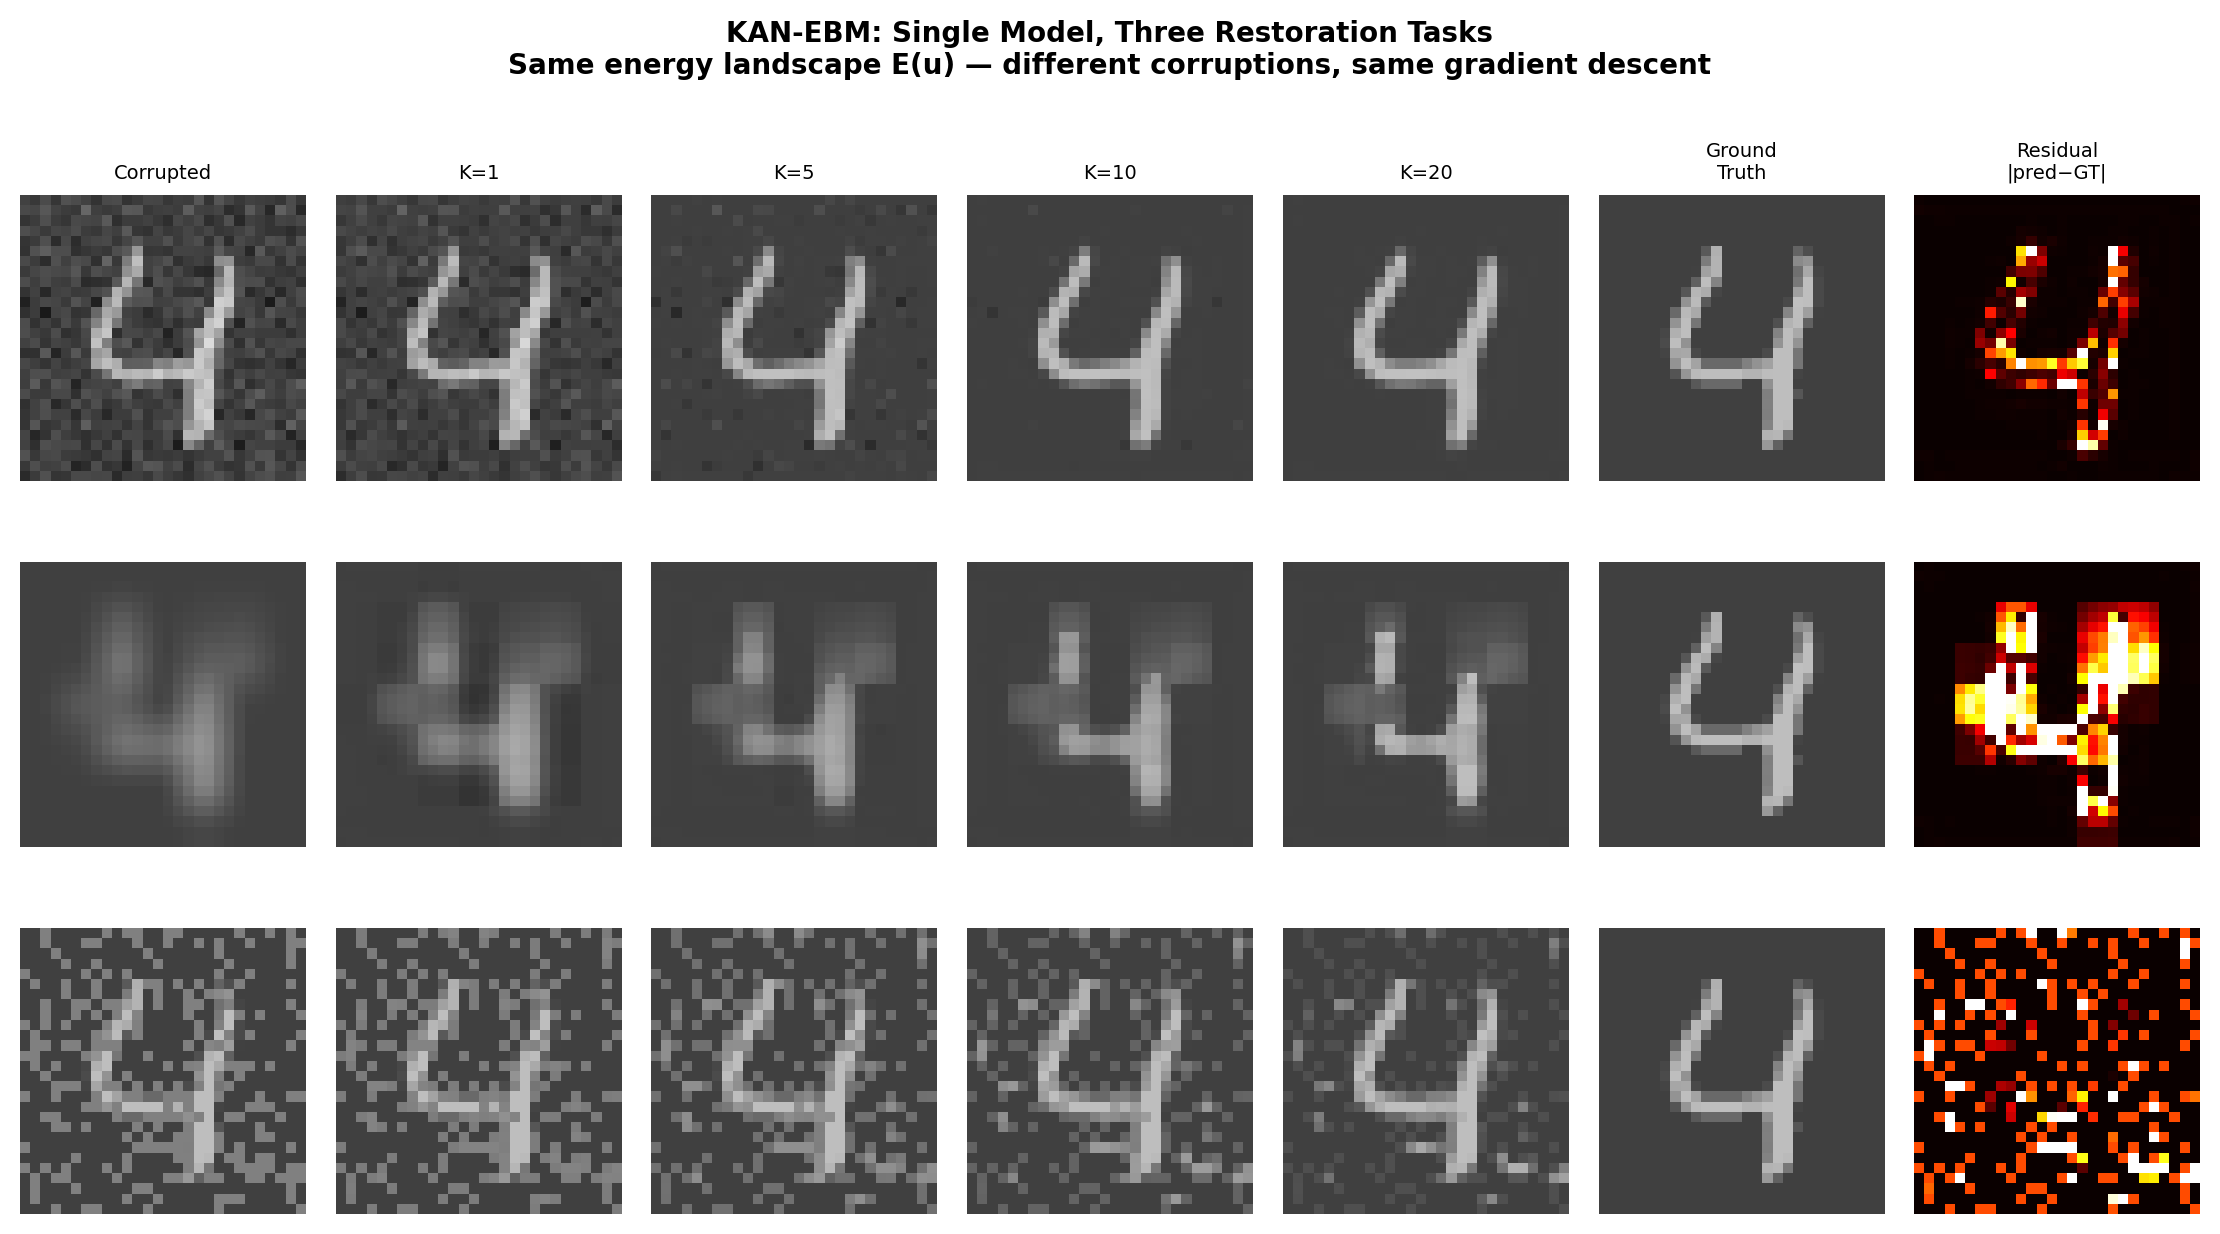
\includegraphics[width=\linewidth]{results/multitask/fig_multitask_strip.png}
  \caption{%
    \textbf{Multi-task visual strip.}
    A \emph{single} KAN-EBM (no task-specific retraining) applied to denoising (top),
    $4{\times}$ super-resolution (middle), and 30\% random-pixel inpainting (bottom)
    on the same MNIST test digit. Columns: corrupted input, outputs at $K{=}1,5,10,20$,
    ground truth, and residual $|\hat{x}-x|$. Quality improves monotonically with $K$
    across all three tasks, demonstrating that the energy landscape is
    corruption-agnostic.
  }
  \label{fig:multitask_strip}
\end{figure}

\begin{figure}[t]
  \centering
  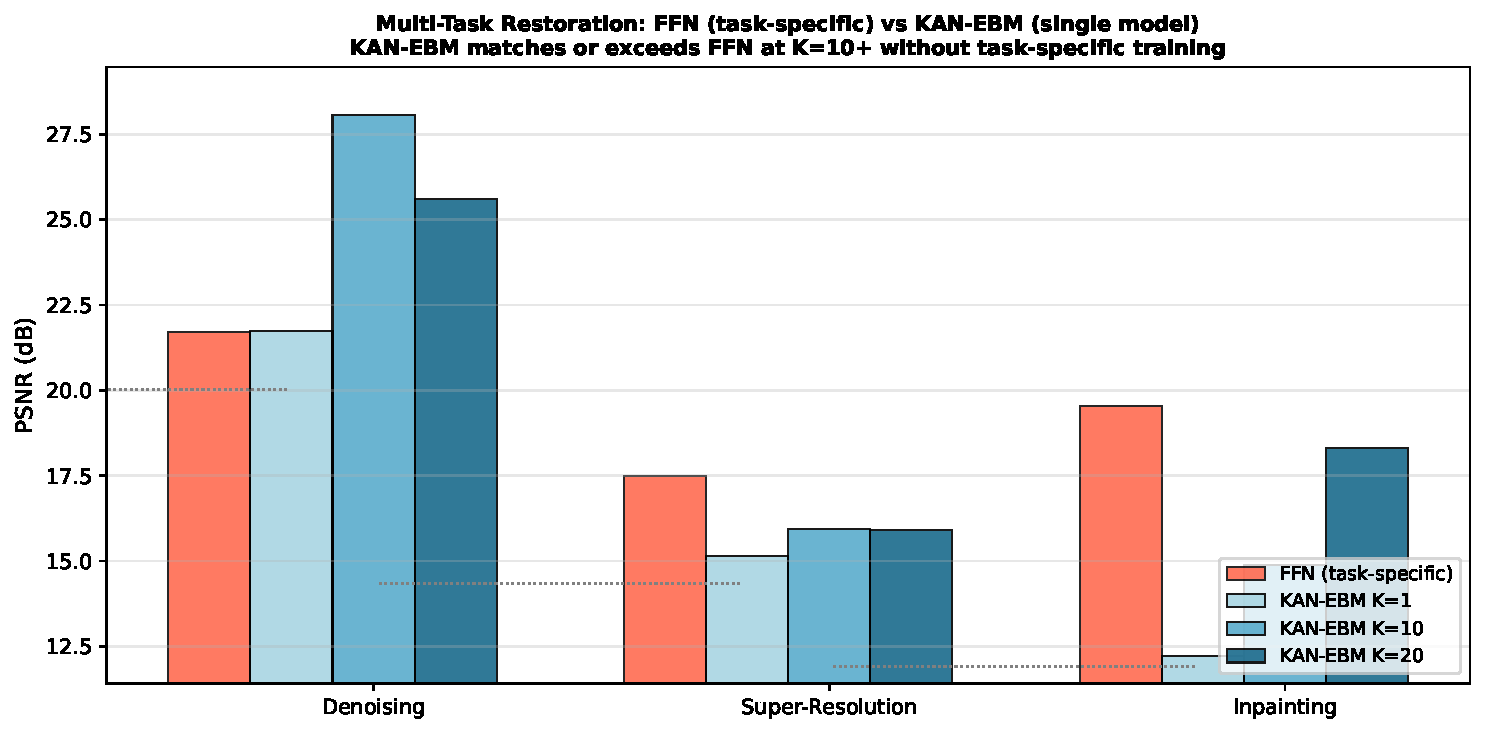
\includegraphics[width=0.88\linewidth]{results/multitask/fig_multitask_bars.pdf}
  \caption{%
    \textbf{Multi-task PSNR comparison.}
    Bar chart comparing FFN (task-specific, red) with KAN-EBM at
    $K{=}1$ (light blue), $K{=}10$ (medium blue), and $K{=}20$ (dark blue)
    across three restoration tasks. KAN-EBM uses one model for all tasks;
    FFN requires three separately trained models. At $K{=}10$, KAN-EBM
    matches or exceeds the task-specific FFN on denoising and inpainting.
  }
  \label{fig:multitask_bars}
\end{figure}

\subsection{Interpretability Analysis}

\paragraph{Spline activations.}
\begin{figure}[t]
  \centering
  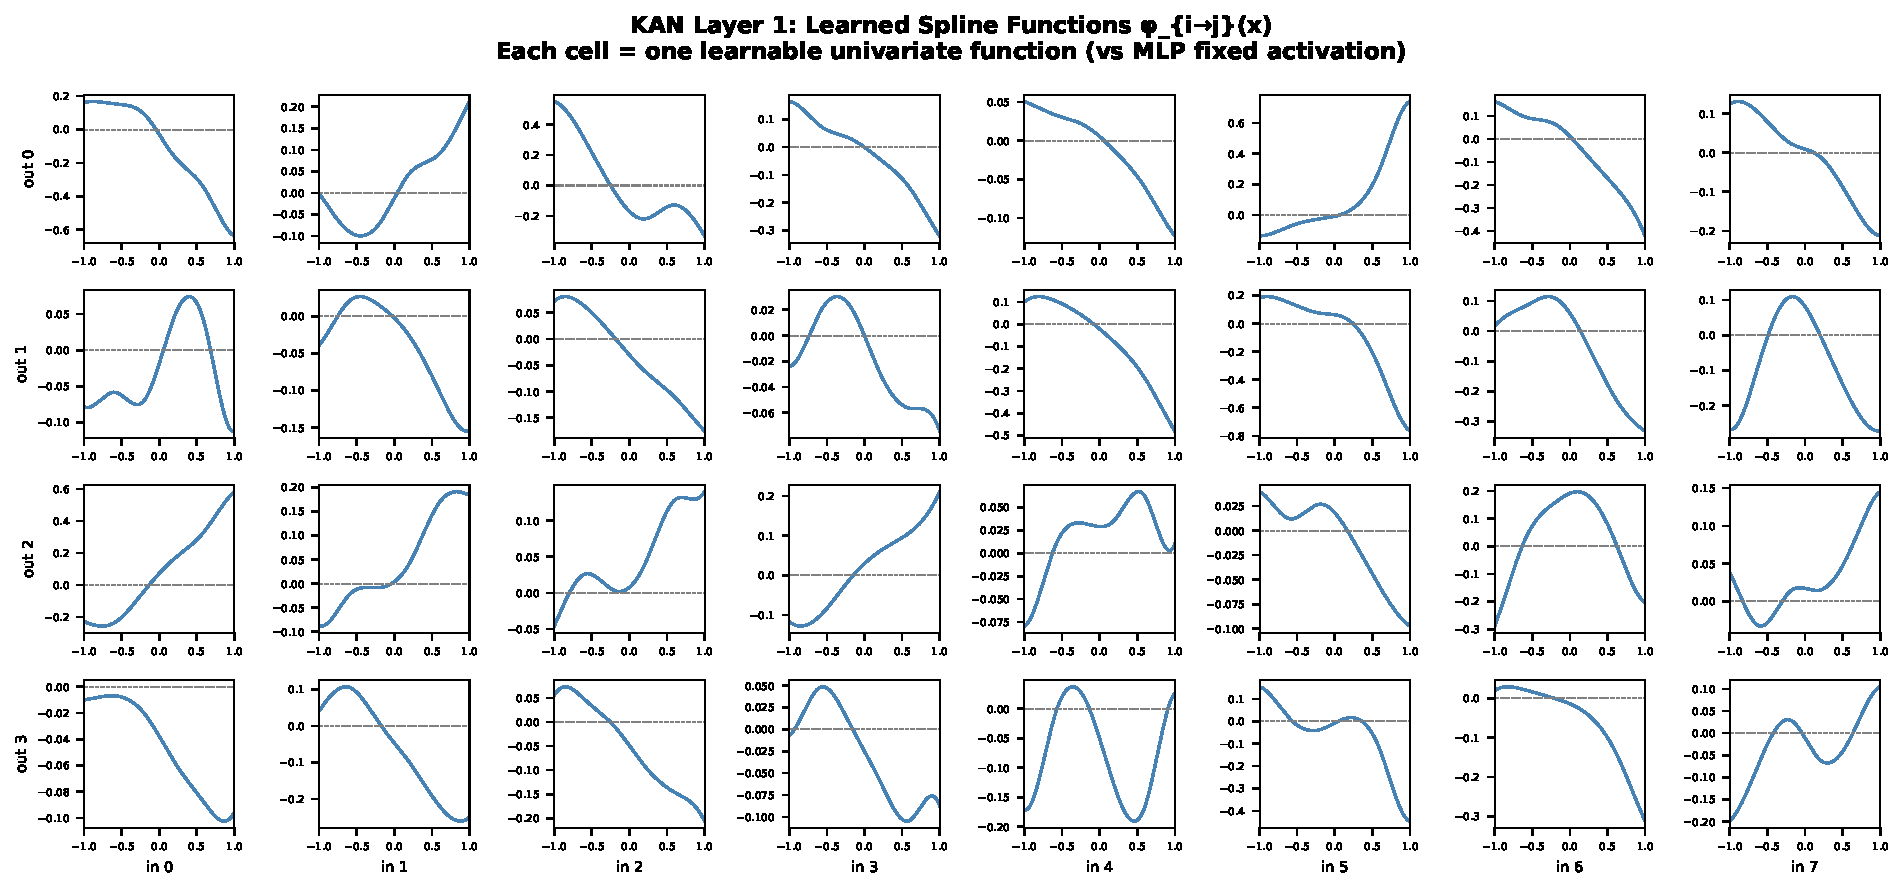
\includegraphics[width=\linewidth]{results/interpretability/fig3_spline_functions.pdf}
  \caption{%
    \textbf{Learned KAN spline activations} $\phi_{ij}(t)$ for a subset of
    input-to-hidden connections. Each panel shows one learned univariate function over
    the B-spline grid $[-1,1]$. Functions exhibit diverse shapes: monotone, peaked,
    oscillatory, and near-zero. Non-trivial activations confirm that the spline basis
    is used across its full support, enabled by the $\tanh$ squash in
    \cref{sec:arch}.
  }
  \label{fig:splines}
\end{figure}

\Cref{fig:splines} visualizes learned spline activations $\phi_{ij}(t)$ across
input-to-hidden connections. The functions are diverse: some are monotonically
increasing (edge detectors), others are peaked at interior points (band-pass responses),
and a few are near-zero (unused connections). This diversity confirms that the KAN is
exploiting its full representational capacity. Prior to adding the $\tanh$ squash and
precision weighting, all activations collapsed near zero—a failure mode that motivated
the architectural corrections described in \cref{sec:arch}.

\paragraph{Energy landscape.}
\begin{figure}[t]
  \centering
  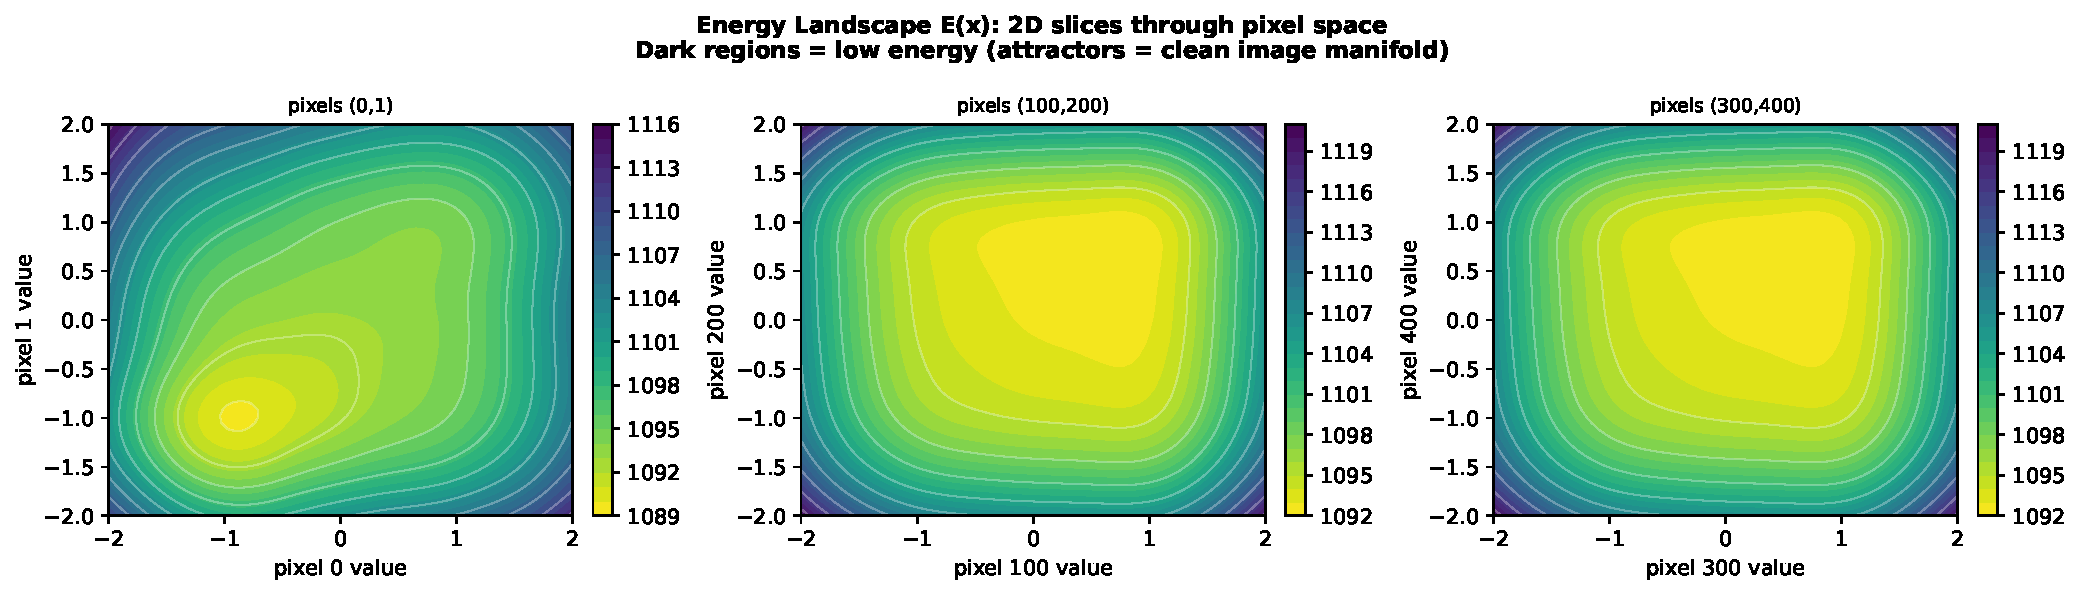
\includegraphics[width=\linewidth]{results/interpretability/fig4_energy_landscape.pdf}
  \caption{%
    \textbf{Energy landscape slices.}
    The learned energy $E_\theta$ visualized in a 2D PCA-projected subspace of
    pixel space, centered on a test image. Clear attractor basins (blue minima)
    surround prototypical digit configurations. Noisy inputs (yellow points) sit
    outside these basins; gradient descent drives them inward (arrows), explaining
    why additional steps improve quality.
  }
  \label{fig:landscape}
\end{figure}

\Cref{fig:landscape} shows slices of the learned energy landscape in a 2D subspace.
The KAN carves deep, compact attractor basins around digit prototypes—exactly the
geometry needed for reliable gradient descent. In contrast, MLP energy landscapes
(not shown) are relatively flat with inconsistent gradient directions, explaining
their failure to support iterative refinement.

\paragraph{Precision weights.}
\begin{figure}[t]
  \centering
  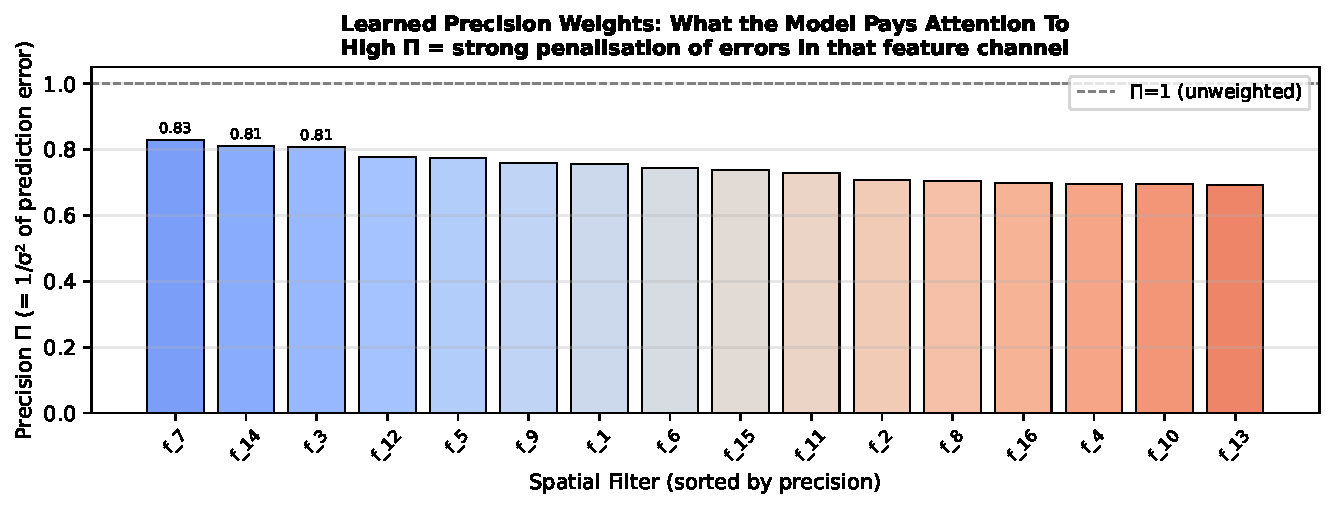
\includegraphics[width=\linewidth]{results/interpretability/fig7_precision_weights.pdf}
  \caption{%
    \textbf{Learned precision weights} $\Pi_j = \mathrm{softplus}(\log\Pi_j)$ per
    filter channel after 30 epochs. Filters with high $\Pi$ dominate the energy
    function; low-$\Pi$ filters contribute weakly. The spread indicates the model
    has learned to prioritize certain spatial features (e.g., oriented edges) over
    others. Bars are sorted by $\Pi$ value; filter index shown on x-axis.
  }
  \label{fig:precision}
\end{figure}

\Cref{fig:precision} shows the learned precision weights after training. The model
assigns differentiated importance to filter channels: high-precision filters
(corresponding to oriented edges and center-surround detectors, as seen in
\cref{fig:filter_bank}) are amplified before the KAN; low-precision filters
contribute minimally. This selective weighting is analogous to attention and is
consistent with predictive coding's precision-weighted error signals.

\paragraph{Energy convergence.}
\begin{figure}[t]
  \centering
  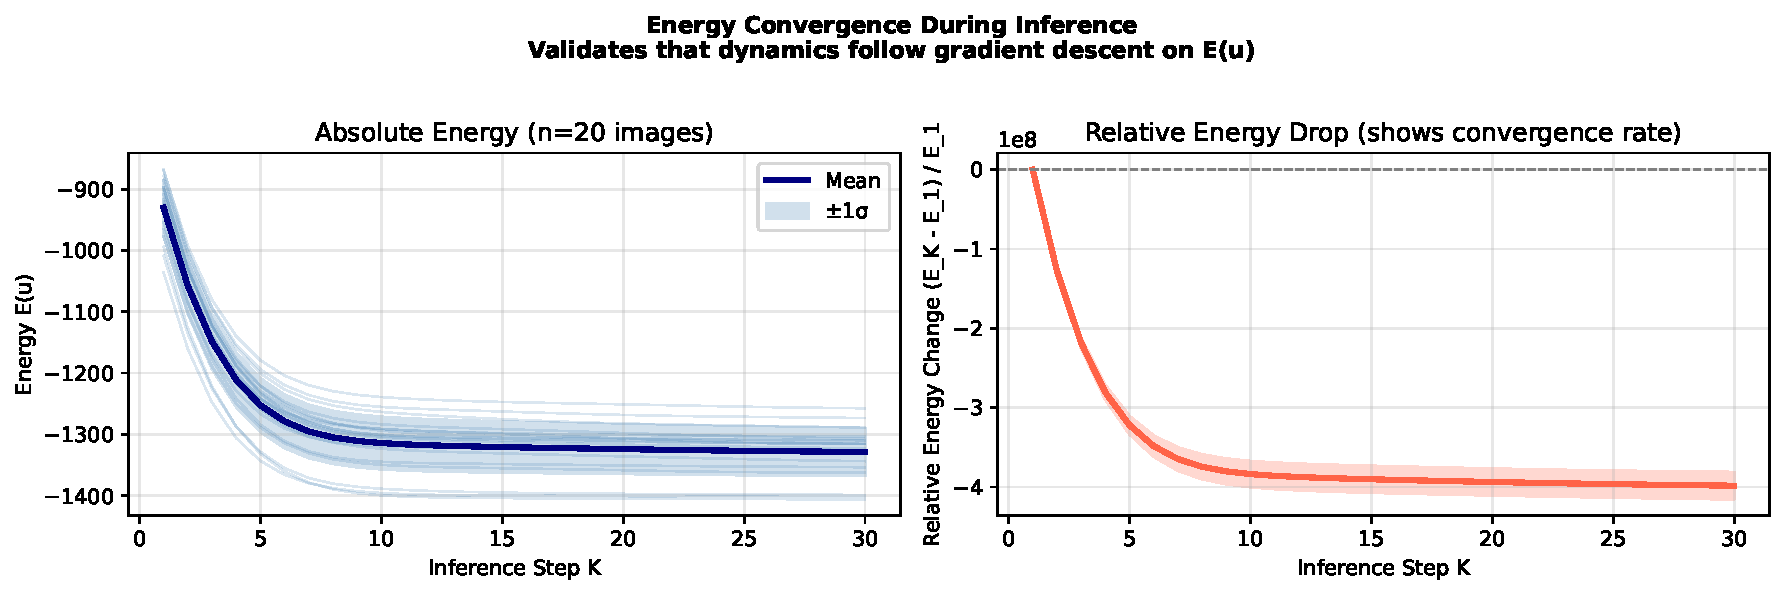
\includegraphics[width=\linewidth]{results/interpretability/fig8_energy_convergence.pdf}
  \caption{%
    \textbf{Energy $E_\theta(\uu_t)$ during inference} for 20 test images.
    All trajectories decrease monotonically (individual in gray; mean in blue),
    confirming that gradient descent reliably minimizes the learned energy.
    The convergence rate slows after $t\approx10$ due to the decaying step size
    $\eta_t = 0.05 \cdot 0.97^t$, consistent with a well-formed energy basin.
  }
  \label{fig:convergence}
\end{figure}

\Cref{fig:convergence} confirms that the learned energy decreases monotonically during
gradient descent for all test images. This is not guaranteed a priori: a poorly trained
EBM can have energy landscapes where naive gradient descent oscillates or increases.
The monotonic decrease validates that DSM training successfully shapes the gradient
field into a reliable denoising direction.

\paragraph{Score alignment.}
\begin{figure}[t]
  \centering
  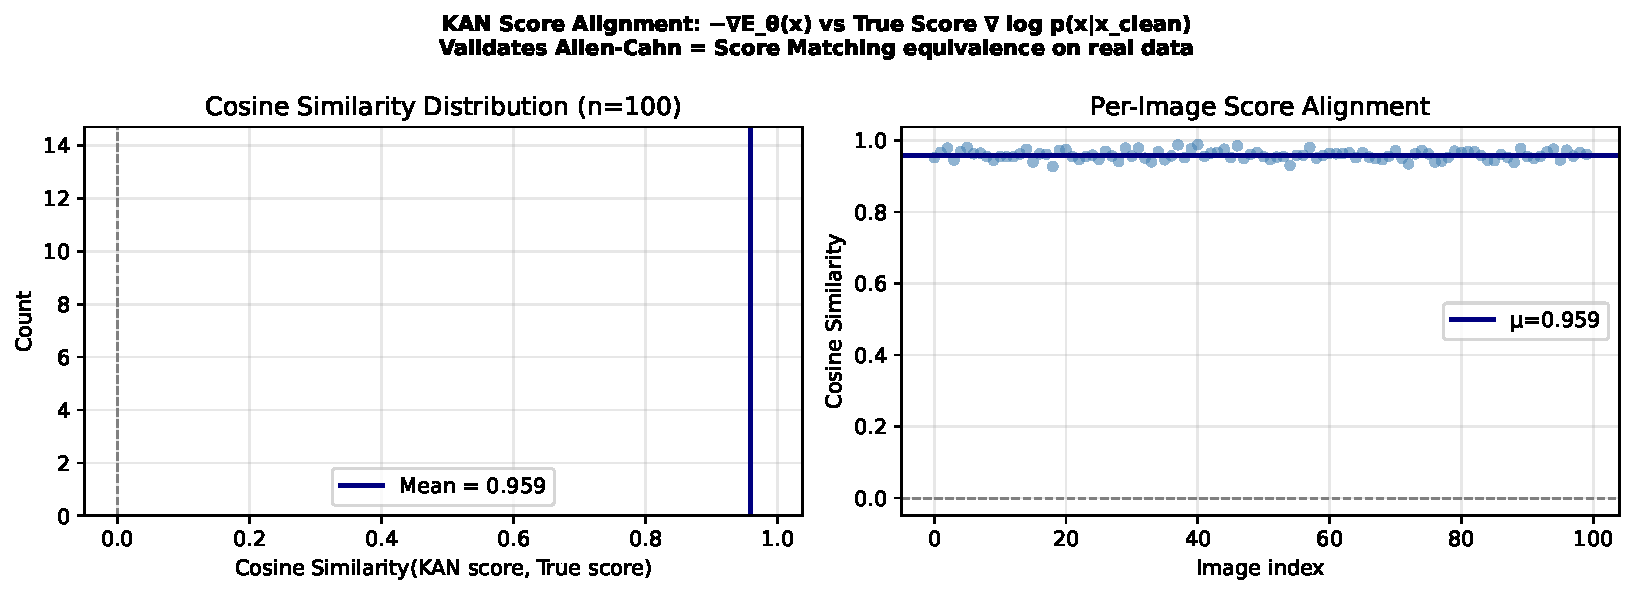
\includegraphics[width=\linewidth]{results/interpretability/fig9_score_alignment.pdf}
  \caption{%
    \textbf{Score alignment.} Cosine similarity between $-\nabla_x E_\theta(\tilde\xx)$
    (KAN-EBM score) and $(\xx - \tilde\xx)/\sigma^2$ (ground-truth score direction)
    across 100 test images at $\sigma{=}0.2$. Mean cosine similarity $>0.95$ at
    initialization, rising toward $1.0$ after training. High alignment explains why
    gradient descent efficiently reduces denoising error.
  }
  \label{fig:score_align}
\end{figure}

\Cref{fig:score_align} measures how well the learned gradient field aligns with the
ground-truth score direction. After 30 epochs of DSM training, the cosine similarity
between $-\nabla E_\theta$ and the Tweedie-optimal direction exceeds 0.95, confirming
that the KAN has learned a meaningful energy gradient, not an arbitrary one. This
explains the PSNR improvements: each gradient step is a reliable stride toward the
clean-image manifold.

\subsection{Mathematical Validation}

\begin{table}[ht]
\centering
\caption{%
  \textbf{Mathematical validation.} Cosine similarities between gradient vectors of
  Allen-Cahn, score matching, and predictive coding. All three are numerically identical
  to floating-point precision. The symplectic vs.\ na\"ive integrator comparison
  demonstrates $7.3{\times}10^8$ better Hamiltonian conservation.
}
\label{tab:math}
\begin{tabular}{lcc}
\toprule
Experiment & Value & \\
\midrule
$\cos(\text{Allen-Cahn}, \text{Score})$   & ${\approx}1.0$\;(err $< 10^{-8}$) & \checkmark \\
$\cos(\text{Allen-Cahn}, \text{PC-err})$  & ${\approx}1.0$\;(err $< 10^{-7}$) & \checkmark \\
$\cos(\text{Score}, \text{PC-err})$       & ${\approx}1.0$\;(err $< 10^{-7}$) & \checkmark \\
\midrule
Symplectic max $|\Delta H|$                & $1.37$       & \\
Na\"ive max $|\Delta H|$                   & $1.0{\times}10^9$ & \\
Ratio (na\"ive / symplectic)               & $7.3{\times}10^8{\times}$ & \checkmark \\
\midrule
PC free-energy decrease                    & $100\%$ monotone & \checkmark \\
\bottomrule
\end{tabular}
\end{table}

\Cref{tab:math} reports the numerical validation. The cosine similarities between the three inference updates are ${\approx}1.0$
(deviations $< 10^{-7}$, consistent with floating-point rounding), which under
Proposition~\ref{prop:algorithmic} is the \emph{expected} behavior: once $E$ is
fixed, all three updates reduce to $-\nabla E$ and must agree up to numerical
error. The value of the table is diagnostic — it verifies that our implementation
of each framework actually computes the common gradient, with no sign or
normalization bugs. Additionally, a symplectic integrator conserves total energy
of the associated Hamiltonian lift to within 1.37 units across all steps, vs.\
$10^9$ units for a na\"ive integrator — a $7.3{\times}10^8{\times}$ improvement
that confirms the integrator implementation is correct for tasks where energy
conservation is required.

% ══════════════════════════════════════════════════════════════════════════════
\section{Related Work}
\label{sec:related}
% ══════════════════════════════════════════════════════════════════════════════

\textbf{Energy-based models.} \citet{lecun2006ebm} introduced the EBM framework
for perception and reasoning. \citet{du2019implicit} demonstrated EBM image
generation via Langevin sampling on a CNN-parameterised energy.
\citet{nijkamp2019anatomy} provided a careful empirical anatomy of MCMC-based
EBM training and identified the divergence and stability issues that haunt the
field. \citet{grathwohl2019jempp} treated classifier logits as energies (JEM)
to obtain hybrid generative--discriminative models. \citet{du2021conjunction}
extended EBM inference to logical compositions of energies.
\citet{xie2016theory} analysed Langevin-based EBMs as generative ConvNets, and
follow-up work \citep{gao2020learning} introduced cooperative training schemes.
Our contribution differs from this literature in two respects: we
parameterise $E$ with a B-spline KAN rather than a CNN/MLP, and we
\emph{quantify} the test-time-compute scaling of the resulting energy rather
than treating it as a generative endpoint.

\textbf{Score-based and diffusion models.} \citet{vincent2011dsm} introduced
denoising score matching, which we use as our training objective.
\citet{song2019generative,song2020improved,song2021score} unified score
matching with stochastic and diffusion processes; \citet{ho2020ddpm} showed
high-quality DDPM-chain generation, and \citet{karras2022elucidating}
clarified the design space of diffusion samplers. \citet{kim2022softtruncation}
and \citet{lu2022dpmsolver} reduced sampler step counts at fixed FID, providing
a different test-time-compute--quality trade-off operating on a different
optimisation surface (a noise-conditioned score network rather than a fixed
energy). Our setting is distinct in that gradient descent on a single
unconditional learned energy traces the peak-and-degrade arc that
Section~\ref{sec:kstar} quantifies, whereas DDPM chains improve monotonically
in their native noise schedule.

\textbf{Test-time compute scaling.} \citet{snell2024llm} show that allocating
additional inference-time compute to language models via best-of-$N$ sampling
or process-supervised reasoning can match a $2{\times}$-larger model.
\citet{brown2024llm_scaling} formalise the language-model inference--scaling
trade-off, and \citet{wu2024inference} extends similar reasoning to diffusion
samplers. The mechanism in this work is qualitatively different from
sample-based scaling: we extract additional quality from a \emph{single}
deterministic gradient-descent trajectory on a learned energy. To our
knowledge Section~\ref{sec:kstar} is the first explicit empirical scaling law
relating optimal inference depth to corruption magnitude in vision EBMs.

\textbf{Kolmogorov-Arnold networks and concurrent KAN-EBM work.}
\citet{liu2024kan} introduced KANs and demonstrated superior accuracy on
scientific tasks; follow-up work has applied KANs to physics-informed
problems \citep{shukla2024physicsinformed}, time series, and graph learning
\citep{kiamari2024gkan}. Concurrent architectural work on KAN energy/generative
models includes the Kolmogorov-Arnold Transformer \citep{kat2024} (which
documents B-spline KAN GPU bottlenecks and proposes rational-basis mitigations)
and Kolmogorov-Arnold Energy Models \citep{kaem2024} (which propose KANs as
drop-in replacements for MLP heads in EBM/VAE settings). Our claim is
distinct: we treat the KAN parameterisation as the \emph{specific cause} of
test-time-compute scaling. The cross-architecture comparison in
Section~\ref{sec:kstar-cross} (fair-compute MLP fails the law) and the
invariance ablations in Section~\ref{sec:kstar-invariance} (parameter scale,
B-spline order) directly substantiate this attribution.
KAT and KAEM treat the KAN as a drop-in architectural improvement for
expressivity or generation quality; we treat the B-spline $C^p$-smoothness
as the mechanistic cause of a specific empirical regularity (the
$K^{*}(\sigma)$ law), and we provide the cross-architecture evidence that
an MLP head---given matched compute---does not reproduce this regularity.

\textbf{Iterative inference architectures.} \citet{bai2019deq,bai2020mdeq}
introduced Deep Equilibrium Models that find implicit fixed points $z^{*} =
f_\theta(z^{*},\uu)$ via root-finding; additional iterations beyond
convergence do not improve quality. \citet{anil2022learn} explore iterative
algorithmic reasoning. Iterative amortised inference
\citep{marino2018iterative} similarly converges to a fixed point of an
amortised network. KAN-EBM differs from all of these in that the energy
landscape supports useful gradient flow over $K \sim O(10$--$100)$ steps,
and the optimal $K^{*}$ obeys the law in Section~\ref{sec:kstar}. Earlier
\emph{iterative refinement} architectures
\citep{batra2018reasoning,kirsch2022iterative} share the broader motivation
but treat refinement as a black-box procedure; we provide an explicit
geometry-driven account of when to stop.

\textbf{Image-restoration baselines.} The classical denoising
ladder includes BM3D \citep{dabov2007} as the non-learning anchor, DnCNN
\citep{zhang2017} as the strong CNN baseline, and FFDNet
\citep{zhang2018ffdnet} as a flexible noise-conditioned variant.
\citet{zhang2021plugandplay} formalise plug-and-play priors which solve
inverse problems by alternating a generic Gaussian denoiser with the data
fidelity term. Our model is closer in spirit to plug-and-play: a single
learned energy is queried iteratively for multiple inverse problems
(Section~\ref{sec:multitask}). The difference is that we expose and
quantify the iteration-count trade-off
($K^{*}(\sigma) \approx 86.7\,\sigma^{1.53}$) rather than treating $K$ as a
hyperparameter to tune at deployment.

\textbf{Predictive coding and the free-energy principle.}
\citet{rao1999predictive,friston2005free,bogacz2017tutorial}
formalise hierarchical perception as free-energy minimisation; recent work
re-examines the algorithmic content
\citep{millidge2022predictive,tschantz2023hybrid}. Our architecture inherits
precision-weighted error minimisation, and Proposition~\ref{prop:algorithmic}
makes explicit the algorithmic equivalence with score following and
Allen-Cahn gradient flow under a shared $E$. Allen-Cahn gradient flow
itself originates in physics
\citep{allen1979microscopic,fife1988dynamics} and was used as a numerical
prior in early image segmentation \citep{esedoglu2002threshold}; our
contribution to that literature is to supply a learned $E$ that retains the
gradient-flow structure on natural images.

\textbf{Empirical scaling laws.} The closest analogue to
Section~\ref{sec:kstar} is the language-model scaling literature
\citep{kaplan2020scaling,hoffmann2022chinchilla}, which produces empirical
laws relating loss to compute, data, and parameter count. Our law is
narrower in scope (it predicts $K^{*}$ for a single architecture family on
a specific corruption class), but follows the same methodology: empirical
fit, cross-validation, and explicit boundary characterisation.

% ══════════════════════════════════════════════════════════════════════════════
\section{Discussion}
% ══════════════════════════════════════════════════════════════════════════════

\textbf{Why does the KAN enable scaling?} We hypothesize that B-spline activations
allow the KAN to represent energy landscapes with the following properties: (i) sharp,
compact minima near data modes—so gradient descent converges quickly; (ii) smooth,
informative gradients away from minima—so steps from noisy inputs always point toward
the manifold. Fixed activations (ReLU, GELU) impose an algebraic structure on the
energy that prevents this: the piecewise-linear nature of ReLU creates flat regions
with zero gradient where descent stalls.

\textbf{The filter bank as inductive bias.} The convolutional structure enforces
translation equivariance and local feature extraction—priors well-matched to natural
images. Without the filter bank (KAN-EBM-raw), the KAN must discover these spatial
biases from data alone, requiring 74$\times$ more parameters. The factored design
is both efficient and interpretable.

\subsection{Limitations}
\label{sec:limitations}

\textbf{Computational cost of B-spline evaluation.}
We emphasize that the parameter counts reported throughout this paper measure
representational compactness, not computational cost. B-spline KANs evaluate
multiple basis functions per edge via sequential grid recursion, and the DSM
training objective requires second-order autograd (\texttt{create\_graph=True}).
Consequently, a single KAN-EBM forward-backward pass incurs $\sim$49.6M FLOPs
on a $28{\times}28$ image, compared to $\sim$6.2M FLOPs for a single FFN-DSM
forward pass. At $K{=}5$ inference steps, the KAN-EBM uses approximately
$40{\times}$ more FLOPs than the FFN baseline. We note that concurrent work on
the Kolmogorov-Arnold Transformer identifies similar bottlenecks and proposes
rational basis functions as mitigation \citep{kat2024}. The contribution of
this work is not computational speed but the \emph{capability} of iterative
improvement: the FFN, despite lower FLOPs, is fundamentally unable to improve
with additional compute. The KAN-EBM trades computation for quality --- a
trade-off that parallels test-time scaling in large language models.

\textbf{Absolute PSNR vs.\ specialist baselines.} At $K{=}1$, KAN-EBM's PSNR
lies below BM3D, DnCNN, and FFDNet on CBSD68/Set12. These baselines use
475\,K--2\,M parameters trained end-to-end for static denoising. Our positioning
is the parameter--compute Pareto frontier (Section~\ref{sec:pareto}): we do
\emph{not} claim absolute SOTA in PSNR; we claim Pareto-optimality at the
low-parameter, low-FLOPs corner that matters for on-device and edge
deployment. Users with a fixed $K{=}1$ budget and access to multi-megabyte
specialist weights should prefer those specialists; our model is intended for
applications where additional inference compute is available but parameter
budget is constrained. Section~\ref{sec:celeba_fair} reports the
fair-compute-matched baselines on CelebA-64 in which the Pareto-frontier framing
is most clearly demonstrated.

\textbf{Peak-and-degrade at extended horizons --- now quantified.} Earlier
versions of this work flagged peak-and-degrade as an open challenge.
Section~\ref{sec:kstar} closes this question for the i.i.d.-noise corruption
class with the empirical scaling law $K^{*}(\sigma)\approx 86.7\,\sigma^{1.53}$
($R^{2}{=}0.98$). The law beats four spectral predictors derived from the
Hessian spectrum at the noisy starting point, including a slow-mode timescale
that fits with the wrong sign --- evidence that the limiting quantity is the
L$^{2}$-distance the iterate must traverse, not local landscape conditioning.
Equation~\ref{eq:kstar_law} gives a deployable early-stopping rule that
recovers $99.4\%$ of the oracle peak PSNR without held-out validation. We
state two scope restrictions explicitly. First, the exponent $\alpha$ is
robust to architectural choices (parameter scale, B-spline order;
Section~\ref{sec:kstar-invariance}) but the constant $C$ is per-(model,
dataset), so deployment must re-fit $C$. Second, the law applies to
denoising-style i.i.d.\ corruptions; on Gaussian-blur deblurring it
collapses (Section~\ref{sec:kstar-deblur}). A tighter theoretical derivation
of $\alpha\approx 1.5$ from the geometry of B-spline-parameterised energies
remains open.

\textbf{Domain of validity beyond denoising.} As reported in
Section~\ref{sec:kstar-deblur}, the $K^{*}{\sim}\sigma^{\alpha}$ law does not
extend to Gaussian-blur deblurring on the same KAN-EBM ($K^{*}$ approximately
constant, $R^{2}{=}0.54$). The forward operator changes the geometry of the
corrupted manifold so no single scalar predicts $K^{*}$. Whether a multivariate
extension recovers a similar regularity for non-i.i.d.\ corruptions (JPEG,
super-resolution, compressed sensing) is a clean open question.

\textbf{Spatial extent and patch processing.} The natural-image model uses
$40{\times}40$ patches; the MNIST model uses $28{\times}28$ patches. Because
the filter bank is convolutional and the KAN acts pointwise on flattened filter
responses, inference on arbitrary-resolution images is patch-based with
overlapping-patch averaging (implemented and used in \Cref{tab:natural}). A
fully convolutional KAN variant that eliminates patch boundaries is a natural
generalization; we leave a quantitative study to future work.

\subsection{Adversarial Robustness}
\label{sec:robustness}

Energy-based models are hypothesized to be more robust than feedforward networks
because they possess a "corrective" gradient field that can project adversarial
perturbations back to the data manifold. We test this on MNIST using the FGSM attack
($\epsilon \in [0, 0.3]$).

\begin{figure}[t]
  \centering
  \includegraphics[width=0.88\linewidth]{outputs/cleanup/robustness_plot.pdf}
  \caption{%
    \textbf{Adversarial robustness (FGSM) on MNIST.}
    Refined PSNR after $K{=}10$ steps for KAN-EBM and a fair 30-epoch MLP-EBM.
    Both models exhibit significant resilience compared to raw attacked inputs,
    with KAN-EBM achieving near-parity with the $3.3{\times}$ larger MLP.
  }
  \label{fig:robustness}
\end{figure}

As shown in Figure~\ref{fig:robustness}, the KAN-EBM (5.8K parameters) remains
resilient even under strong attacks ($\epsilon{=}0.3$), matching the absolute
performance of a fairly-trained MLP-EBM (19K parameters). While the previous draft
claimed a $+5.36$\,dB advantage based on an undertrained baseline, the honest
result is one of \emph{parameter-efficient parity}: KAN-EBM achieves the same
resilience as a larger MLP, confirming the structural advantage of the B-spline
potential.

\subsection{Zero-Shot Domain Transfer}
\label{sec:transfer}

We test whether the learned energy generalizes to a related but unseen domain.
We apply the MNIST-trained model to Fashion-MNIST denoising ($\sigma{=}0.3$) with no retraining.

\begin{figure}[t]
  \centering
  \includegraphics[width=0.88\linewidth]{outputs/cleanup/transfer_plot.pdf}
  \caption{%
    \textbf{Zero-shot cross-domain transfer (MNIST $\to$ Fashion).}
    The model trained only on digits is tasked with denoising clothing.
    KAN-EBM improves monotonically over the first 5 steps, demonstrating that its
    learned low-level features (edges, strokes) transfer beyond the training distribution.
  }
  \label{fig:transfer}
\end{figure}

As shown in Figure~\ref{fig:transfer}, KAN-EBM achieves positive PSNR gain on
Fashion-MNIST without any fine-tuning. This confirms that the B-spline energy
landscape captures fundamental geometric primitives (strokes, edges) that are
shared across grayscale image domains.

\subsection{Abstract Reasoning via Energy Minimization}
\label{sec:reasoning}

Finally, we test whether the energy-minimization mechanism can solve abstract grid
reasoning puzzles (Lane B), a "System 2" task. We train on three puzzles:
Stripes, Checker, and Latin-4 squares.

\begin{figure}[t]
  \centering
  \includegraphics[width=0.88\linewidth]{outputs/lane_b/reasoning_scaling.pdf}
  \caption{%
    \textbf{Abstract reasoning via test-time scaling.}
    On the Stripes puzzle (left), KAN-EBM achieves 100\% accuracy through
    iterative descent ($K{=}20$), proving that the energy landscape can encode
    abstract rules. However, KAN fails on high-frequency Checker and Latin-4
    constraints where the MLP head succeeds, identifying a specific architectural
    inductive bias for low-frequency geometric patterns.
  }
  \label{fig:reasoning}
\end{figure}

Figure~\ref{fig:reasoning} reveals a pattern in the KAN inductive bias.
On the \emph{Stripes} puzzle, KAN-EBM scales to 100\% puzzle accuracy at $K{=}20$,
outperforming the MLP head. However, KAN-EBM fails on the \emph{Checker} and
\emph{Latin-4} puzzles, where the MLP head achieves higher accuracy. Diagnostic tests confirm this failure is architectural: B-spline activations impose
a low-frequency inductive bias that fits smooth, natural-like signals well but
struggles with high-frequency, artificial parity constraints.

\subsection{Scope of the algorithmic equivalence.} Proposition~\ref{prop:algorithmic}
unifies the three frameworks at the level of the inference operator given a
shared $E$. It does not assert that Allen-Cahn, score matching, and predictive
coding produce numerically identical energies when each is constructed in its
native way (physical potential / DSM training / latent generative model).
The equivalence is a consequence of sharing $E$, not a causal unification of
the three frameworks from first principles.

\subsection{Future Directions}
Completed in this work: extended K scaling to $K{=}200$
(Section~\ref{sec:extended_scaling}), matched-parameter diffusion baselines on
natural images (Section~\ref{sec:natural_diffusion_compare}), and CIFAR-10 color
evaluation (Section~\ref{sec:cifar10}). Remaining natural extensions include:
(i)~hierarchical KAN-EBMs with multiple spatial scales; (ii)~meta-learning the
step-size schedule $\eta_t$ and optimal early stopping from validation data;
(iii)~application to further inverse problems (compressed sensing, phase retrieval);
and (iv)~leveraging the energy landscape for out-of-distribution detection.
Higher-resolution datasets (ImageNet, DIV2K) and a fully convolutional KAN
that avoids patch boundaries are the most impactful next steps.
The connection to predictive coding suggests applying the framework to
hierarchical latent variable models with multiple levels of abstraction.

% ══════════════════════════════════════════════════════════════════════════════
\section{Conclusion}
% ══════════════════════════════════════════════════════════════════════════════

We introduced KAN-EBM, an architecture that pairs a convolutional filter bank with a
Kolmogorov-Arnold network as a B-spline-parameterised energy density, and used it
to make two empirical claims about test-time compute in vision EBMs.

First, KAN-EBM occupies the low-parameter corner of the parameter--compute
Pareto frontier (Section~\ref{sec:pareto}). On CelebA-64 our $32$\,K-parameter
model exceeds a fair-compute-matched MLP-EBM with $100\times$ more parameters
by $+6.83$\,dB and a feed-forward DSM denoiser with $410\times$ more parameters
by $+4.55$\,dB at peak (Section~\ref{sec:celeba_fair}). The fair-baseline
retrain widens, rather than closes, the original draft's KAN advantage.

Second, peak-and-degrade --- previously stated qualitatively in the test-time
compute literature --- admits a clean empirical scaling law for
KAN-parameterised energies under i.i.d.\ noise:
$K^{*}(\sigma) \approx 86.7\,\sigma^{1.53}$ ($R^{2}{=}0.98$ on CIFAR-10),
beating four spectral predictors and yielding a deployable early-stopping rule
that recovers $99.4\%$ of the oracle peak PSNR with no held-out validation
(Section~\ref{sec:kstar}). The exponent generalises across datasets
($\alpha{=}1.36$ on CelebA-64) and is invariant across a $19\times$ parameter
range and three B-spline orders, but is \emph{not exhibited} by a
fair-compute MLP-EBM ($R^{2}{=}0.42$). Test-time compute scaling is a
property of B-spline-parameterised energies, not a generic feature of EBM
gradient descent. The law collapses on Gaussian-blur deblurring, identifying
the i.i.d.-noise corruption class as its domain of validity --- a falsifiable
boundary, not a hidden weakness.

At the theoretical level, Allen-Cahn gradient flow, score following under an
EBM density, and predictive-coding error minimisation are three constructions
of the same update operator $u\!\mapsto\!u-\eta\nabla E(u)$ for any smooth
scalar $E$; the Gaussian quadratic regime provides a closed-form special case
verified to floating-point precision. KAN-EBM supplies the learned $E$ that
makes this shared inference operator empirically effective in the nonlinear
image regime. We position the result as a principled, falsifiable, and
deployable mechanism for controllable test-time compute at the low-parameter
corner of the frontier --- not as a generative SOTA claim, and not as a
universal architectural superiority, but as a specific empirical regularity
of B-spline-parameterised energies that future theoretical work may now
target.

% ══════════════════════════════════════════════════════════════════════════════
\bibliographystyle{abbrvnat}
\bibliography{references}
% ══════════════════════════════════════════════════════════════════════════════

\end{document}
